\chapter{Anomaly detection in multi-factor data} \label{sec:chapter_sgvaegan}

\section{Introduction}

In the course of this text, we have been gathering information about state-of-the-art methods, available datasets, and potential unsolved problems in anomaly detection. The ultimate goal of this endeavour was to find an intriguing anomaly detection problem and propose a novel method for its solution, which will be presented in this chapter. Here is a list of the findings that have been gathered so far.

\begin{enumerate}
    \item In Section~\ref{sec:alfven}, the problem of identifying anomalies in high-resolution image data was solved and the two-stage model approach proved to be the most successful. The best models were a combination of a probabilistic autoencoder, which produced informative latent encoding, and a classical anomaly detector, which operated on the encoded data of highly reduced dimensionality. The dimensionality reduction alleviated the computational burden from the second stage model which could be more deeply fine-tuned. Eventually, a simple kNN detector was the best choice for a second-stage model. 
    \item In Chapter~\ref{sec:chapter_comparison}, a thorough comparison of existing anomaly detectors was done. We have seen what are the most important contexts of an anomaly detection problem (data type, number of labeled anomalies, and budget available for hyperparameter tuning) that one should consider when choosing a method for solving a practical problem. It was shown that deep generative models gain an edge over other methods when solving anomaly detection problems on image data, especially on problems where semantic anomalies occur. 
    \item In the same chapter, it was shown that although probabilistic autoencoders are generally well-suited for image anomaly detection problems, adversarial training might be beneficial for the detection of \textbf{semantic} anomalies~\cite{ahmed2020detecting} with enough budget for hyperparameter tuning. In fact, the majority of the methods compared in Chapter~\ref{sec:chapter_comparison} failed in the detection of semantic anomalies.
\end{enumerate}

Since the detection of semantic anomalies in images is a relatively novel field, we have decided to cover this problem in this chapter using the findings described in the list above. Semantic anomalies appear most often in visual data and their anomality is based on the high-level (semantic) information in the image. For example, an image (used in~\cite{vskvara2021comparison}) can be anomalous because it is blurred, or because it has a different object in the foreground (e.g. plane in the sky instead of a bird in the sky), or different background (e.g. the plane is on a runway, whereas it is usually on the sky). From the point of view of the above definition, they are all anomalies, but the user might be interested in anomalies of a certain type, or they might want the anomalies to be automatically classified according to their type. This difference can only be made based on the high-level, semantic information of an image. A good semantic detector should be also robust to non-semantic shifts~\cite{ahmed2021systematic}, i.e. data-generating factors that are not present in the training data but are not considered anomalous. The detection of semantic anomalies has been previously studied under the name \textbf{subspace} anomaly detection~\cite{raz2002semantic, kriegel2009outlier,rahmani2016randomized}. The idea, as the name suggests, is that the anomaly is not visible in the full input space, where it might be shadowed by noise, but only in the subspace. The subspace is most of the time "axis parallel" or defined in a linear transformation of the input space. Semantic anomalies further generalize this to non-linear transformations.

It seems unlikely in practice that the subspace in which anomalies would be detectable would be aligned with the input space, or with its linear transformation. Contrary, independent components emerge after non-linear projections as shown in~\cite{burgess2018understanding, kim2018disentangling, esmaeili2019structuredhfvae, tschannen2018recent, bai2021contrastively, kim2019bayes, deecke2021transfer}, which motivates this work. Here, we propose to disentangle the input into independent factors, each providing an anomaly score. Ideally, a semantic anomaly and its source would be then better detectable by one of these scores rather than by a score given to the original input. 

In this chapter, the proposed disentanglement into independent factors and the resulting composition of anomaly scores is first theoretically justified. This multi-factor anomaly score is a weighted combination of anomaly scores corresponding to individual factors of the disentangled latent space. In Sec.~\ref{sec:model}, the concrete details (construction, training, and evaluation) of the novel model are described. In the experimental Sec.~\ref{sec:experiments}, the proposed model is extensively compared to baselines on several image benchmarks. It is demonstrated that the model is capable of detecting the factor that is the most likely source of the anomaly in the unsupervised case, and quickly improves with very few labeled samples.

\section{Decomposing the anomaly score} 
\label{sec:theory}
In this section, we will derive a general formula for the computation of the anomaly score of a VAE model for the case when the latent space can be disentangled into independent components. This will be useful as a theoretical foundation of the proposed anomaly detector in Sec.~\ref{sec:model}.

\subsection{Orthogonal generative model} \label{sec:orthogonal_score}
Let us remind ourselves that the VAE (see Sec.~\ref{sec:vanilla_vae}) fits a generative model with data $\vc{x} \in \mathbb{R}^d$
\begin{align}
p_{\vc{\theta}}(\vc{x}) & = \int_{\mathcal{Z}} p_{\vc{\theta}}(\vc{x} \vert \vc{z})p(\vc{z})d\vc{z} & p_{\vc{\theta}}(\vc{x} \vert \vc{z}) & =\mathcal{N}(\vc{x};\vc{\mu}_{\vc{\theta}}(\vc{z}),\vc{\sigma}^{2} \mathbf{I}),\label{eq:vae}
\end{align}
where $p_{\vc{\theta}}(\vc{x}\vert \vc{z})$ is the decoder and the prior on the latent $h$-dimensional variable $z$ is either fixed $p(\vc{z})=\mathcal{N}(0,\mathbf{I})$, or further parametrized $p_{\vc{\theta}}(\vc{z})$, e.g. as in~\cite{tomczak2017vae}. The VAE also includes an encoder $q_{\vc{\phi}}(\vc{z}\vert \vc{x})$ and is optimized by minimization of the ELBO objective~\eqref{eq:elbo3}. 

The above generative model~\eqref{eq:vae} can be rewritten as $\vc{x}=\vc{\mu}_{\vc{\theta}}(\vc{z})+\vc{e}$ where $\vc{e}$ is (usually isotropic) Gaussian noise. This formulation emphasizes the need for marginalization since $\vc{\mu}_{\vc{\theta}}(\vc{z})$ is a random variable of dimension $h$ (same as that of the latent space $\mathcal{Z}$) and noise $\vc{e}$ is a random variable of dimension $d,$ which is the same as the data. Equation~\eqref{eq:vae} therefore marginalizes away random variables corresponding to latent $z.$ Due to this ambiguity, the assignment between $x$ and $z$ is not unique. In fact, for any $\vc{x}$ exists  $\vc{z}'$~\cite{pidhorskyi2018generative, vsmidl2019anomaly} such that \[
\vc{x}=\vc{x}' + +\vc{e}^{\bot} = \vc{\mu}_{\vc{\theta}}(\vc{z}')+\vc{e}^{\bot}
\]
where $\vc{e}^{\bot}$ is the observation noise that lies in the normal space perpendicular to the manifold defined by the decoder mean $\vc{\mu}_{\vc{\theta}}(\vc{z})$. This interpretation implies independence between $\vc{\mu}_{\vc{\theta}}(\vc{z}')$ and $\vc{e}^\bot$, which allows for the approximation 
\begin{equation}
p_{\vc{\theta}}(\vc{x})\approx p(\vc{\mu}_{\vc{\theta}}(\vc{z}'))p(\vc{e}^{\bot}). 
\end{equation}

However, the independence relation was found~\cite{vsmidl2019anomaly} to be sufficiently accurate even for the original noise estimate, $\vc{x}=\vc{x}'+\vc{e}$.  The  probability of the reconstruction $p_{\vc{\theta}}(\vc{x}')$ is given by the change of coordinate formula from $p_{z}(\vc{z})$ (here we use the subscript $_z$ in order to distinguish that the distribution is on the latent space $\mathcal{Z}$), yielding
\begin{align}
p_{\vc{\theta}}(\vc{x})\approx p_{\vc{\theta}}(\vc{x}')p(\vc{e})=p_{z}(\vc{\mu}_{\vc{\theta}}^{-1}(\vc{x}'))\left\vert \frac{\partial \vc{\mu}_{\vc{\theta}}^{-1}(\vc{x})}{\partial \vc{x}}\right\vert p(\vc{e}).\label{eq:pxjacodeco}
\end{align}
A gaussian noise model might be assumed, e.g. $p(\vc{e}) = \mathcal{N}(\vc{x}-\vc{x}',\vc{\sigma}^{2}\mathbf{I})$. In practice, an anomaly score for the orthogonal model $s(\vc{x}) = - \log p_{\vc{\theta}}(\vc{x})$ is computed as
\begin{align}
s(\vc{x}) & = - \log p(\vc{e}) -\log p_{z}(\vc{z})-\log\left\vert \frac{\partial \vc{\mu}_{\vc{\theta}}^{-1}(\vc{x})}{\partial \vc{x}}\right\vert ,\label{eq:jacodeco}
\end{align}
which is essentially the reconstruction error with additional terms.

\subsection{Anomaly in the latent space}
Let's observe how the above generative model changes when we assume the distribution on latent $\vc{z}$ to be multi-modal conditioned by hidden label $y$. This simplification assumes that the latent distribution for normal and anomalous data is different. Let
\begin{equation} \label{eq:pzy}
p_z(\vc{z}\vert y)=p_{n}(\vc{z})^{y}p_{a}(\vc{z})^{1-y},y\in[0,1],
\end{equation}
where $y=1$ for normal data, $y=0$ for anomalies, and $p_n(\vc{z}),p_a(\vc{z})$ are the latent distributions of normal and anomalous data, respectively. Then from~\eqref{eq:jacodeco} we have
\begin{align*}
s(\vc{x} \vert y) & = - \log p(\vc{e}) -y\log p_{n}(\vc{z})  -(1-y)\log p_{a}(\vc{z}) - \log\left\vert \frac{\partial \vc{\mu}_{\vc{\theta}}^{-1}(\vc{x})}{\partial \vc{x}}\right\vert,
\end{align*}
Since $y$ is usually unknown, we will integrate it away by expectation over $y$, 
\begin{align}
\mathbb{E}_{p(y)} \left[  s(\vc{x} \vert y) \right]  = &  - \log p(\vc{e}) - \log\left\vert \frac{\partial \vc{\mu}_{\vc{\theta}}^{-1}(\vc{x})}{\partial \vc{x}}\right\vert \nonumber \\ 
 & - \int_{\mathcal{Y}} y\log p_{n}(\vc{z}) p(y) dy - \int_{\mathcal{Y}} (1-y)\log p_{a}(\vc{z}) p(y) dy \nonumber \\
   \propto & - \log p(\vc{e}) - \log\left\vert \frac{\partial \vc{\mu}_{\vc{\theta}}^{-1}(\vc{x})}{\partial \vc{x}}\right\vert  - \alpha\log p_{n}(\vc{z}) = s(\vc{x}). \label{eq:jacodeco2}
\end{align}
where we assume $\mathbb{E}_{p(y)} \left[  y \right] =\alpha$, and $p_{a}(\vc{z}) \propto 1$, because the probability of an anomaly is assumed to be the same everywhere, which then allows us to drop this term since it is independent of $\vc{x}$.  


Now consider a \textbf{disentagled} model, where the data is generated from multiple independent latent spaces, $\vc{z}=\vc{z}_{1},\ldots,\vc{z}_{l}$, 
\begin{equation} \label{eq:multilatent}
\vc{x}=f(\vc{z}_{1},\ldots,\vc{z}_{l})+\vc{e},
\end{equation}
where each of the latents has distribution $p(\vc{z}_{i})=\mathcal{N}(0,\mathbf{I})$. Using the same derivations, each of the latent spaces $\vc{z}_i$ can be a potential source of different types of anomalies, with hidden labels  $y=(y_{1},\ldots,y_{l})   $. Therefore, instead of~\eqref{eq:pzy},  we have
\begin{equation} 
p(\vc{z}\vert y)= \prod_{i=1}^l p_{n_i}(\vc{z}_i)^{y_i}p_{a_i}(\vc{z}_i)^{1-y_i},y_i\in[0,1].
\end{equation}
Repeating derivation of (\ref{eq:jacodeco2}) for multiple latent variables, the anomaly score becomes
\begin{align} \label{eq:alphadeco}
s(\vc{x}) & = - \log p(\vc{e}) - \log\left\vert \frac{\partial \vc{\mu}_{\vc{\theta}}^{-1}(\vc{x})}{\partial \vc{x}}\right\vert  -  \sum_{i=1}^{l}\alpha_{i}\log p_{n_{i}}(\vc{z}_{i}),
\end{align}
where $\alpha_{i}$ denotes the probability that the latent variable of the $i$th factor is generated from the normal class. In this work, we assume that $\alpha_i$ is not known during training but has to be estimated in the validation stage from examples of anomalous samples.\footnote{Based on the industrial experience of authors, this assumption is safe, i.e. there are usually examples of anomalies, though their diversity might be low.}

The interpretation of the values of $\alpha_i$ will be important later, in Sec.~\ref{sec:model}, where we construct the latent spaces to give them a specific meaning, and in Sec.~\ref{sec:anomaly_detection}, where we describe their fitting. Fitting the values of all $\alpha_i$ on a set of labeled data is equal to estimating the mean of $p(y_i)$ for the given data. This can be interpreted as estimating how likely it is for an anomaly to appear in the $i$-th latent in the context of the current dataset. 

In contrast, for a single data sample, we are more interested in the actual values of $y_i$, which are binary and which determine whether the sample is anomalous in the context of the latent space $i$. Their estimation is equal to the estimation of the distributions $p(y_i \vert \vc{x})$ and will be discussed in Sec.~\ref{sec:anomaly_factor_identification}. 

\section{Shape-guided decomposition} \label{sec:model}
\begin{figure}[ht!]
    \centering
    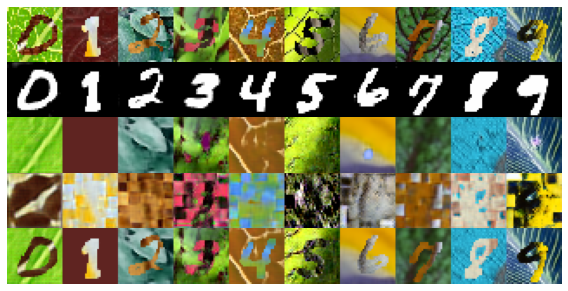
\includegraphics[width=\textwidth]{data/chapter_sgvaegan/fig1_wmnist_grid.png}
    \caption{Examples of decomposition on the Wildlife MNIST dataset by the SGVAEGAN model. The first row contains the input samples, below that are the decoded masks, backgrounds, foregrounds, and finally the whole reconstructions. The model can learn appropriate masks in an unsupervised fashion.}
    \label{fig:wmnist_grid}
\end{figure}

We demonstrate the advantage of disentanglement in detecting semantic anomalies on image data, because (i) the disentanglement has been researched mostly in this domain~\cite{kim2018disentangling, kim2019bayes, choi2020discond}, (ii) the anomaly detection community is the most active in this field, and (iii) the findings of Chapter~\ref{sec:chapter_comparison} showed that most deep generative models are not very efficient when dealing with semantic anomalies.

For the construction of the proposed model, we assume an image $\vc{x}$ to be composed of three main components: a mask (shape of the object), a background texture, and a foreground texture (the object). This of course is not true for all images, but many open datasets contain images that are structured this way. The mask together with the foreground texture defines the semantic meaning of the object, as it is what defines the class of the image in datasets. According to the above assumptions, each component (mask, background texture, and foreground texture) is generated from an independent variable. Therefore, for the latent distribution $p(\vc{z})$ it holds that
\begin{equation} \label{eq:latent_decomposition}
     p(\vc{z}) = p_{z_{m}}(\vc{z}_{m})p_{z_{f}}(\vc{z}_{f})p_{z_b}(\vc{z}_{b}),
\end{equation}
where subscripts $m,f,b$ denote the mask, foreground, and background latent variable, respectively. 
A representative example of a dataset where each image is composed of three independent components is the Wildlife MNIST dataset~\cite{sauer2021counterfactual}. It is constructed using masks from MNIST~\cite{lecun2010mnist} combined with foreground and background textures from~\cite{cimpoi2014describing} (see more details on its construction in Appendix~\ref{sec:appendix_datasets}). For examples from individual classes see the top row of Fig.~\ref{fig:wmnist_grid}. 

The independent decomposition~\eqref{eq:latent_decomposition} is akin to~\eqref{eq:multilatent}, but here we ascribe high-level semantic meaning to the individual latent spaces. This means that the model built on top of the assumption~\eqref{eq:latent_decomposition} has an inductive bias, which enables the unsupervised disentangled representation of the individual components of an image. The independency is further reinforced by the fact that the parts of the model responsible for the representation of the components do not share weights. Furthermore, since we want to apriori ascribe specific meaning to the disentangled latent spaces, we cannot use automatic disentanglement of individual dimensions as is the case in literature~\cite{burgess2018understanding, kim2019bayes, deecke2021transfer}, since there, the disentanglement is not unique and the semantic meaning of the disentangled factors has to be found manually in a post-processing phase.

In this section, the structure of the proposed generative model with independent latent spaces and its training procedure is described first. Then, in order to be able to detect and describe semantic anomalies, we combine the model with the anomaly score derived in Sec.~\ref{sec:theory}.

\subsection{Shape-guided VAEGAN model} \label{sec:sgvaegan}
 \begin{figure}[ht]
    \centering
       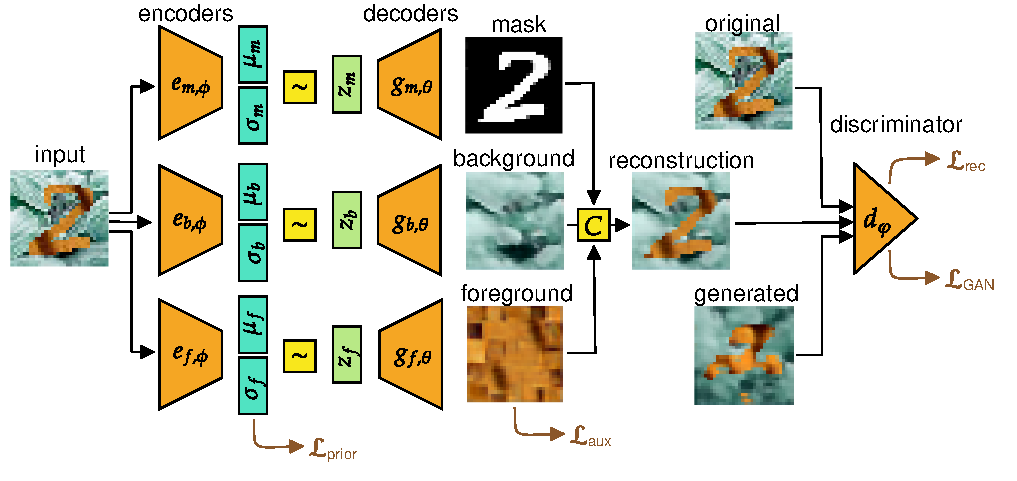
\includegraphics[width=\textwidth]{data/chapter_sgvaegan/fig2_sgvaegan_losses.pdf}
    \caption{The schema of the proposed model. Convolutional blocks are denoted in orange, fully connected in cyan, and intermediate representations in green. The yellow squares represent special operations - $c$ is the composition~\eqref{eq:composition} and the reparametrization trick is denoted by $\sim$. The generated sample is obtained by feeding samples from priors $\mathcal{N}(0,\mathbf{I})$ to the decoders.}
    \label{fig:sgvaegan_schema}
\end{figure}

The model disentangling the input image into its three components is our synthesis of a VAEGAN~\cite{larsen2016autoencoding} and Counterfactual generative networks (CGN)~\cite{sauer2021counterfactual}.\footnote{Counterfactual generative networks~\cite{sauer2021counterfactual} were selected because based on our preliminary experiments, the result offered superior disentanglement likely due to highly inductive bias.} Building blocks of this model, further denoted as SGVAEGAN, are outlined in Fig.~\ref{fig:sgvaegan_schema}. The model uses three separate independent autoencoders for three components of an image, a block combining them to the reconstructed image, and a discriminator for improved performance on semantic image data. We emphasize that it is this strict separation of autoencoders that improves the desired disentanglement.

Autoencoders responsible for individual components are vanilla VAE consisting of an encoder
\begin{equation} \label{eq:encoder}
    q_{i,\vc{\phi}}(\vc{z}_i \vert \vc{x}) = \mathcal{N} \left(\vc{z}_i; \vc{\mu}_{i,\vc{\phi}}(\vc{x}), \text{diag}(\vc{\sigma}_{i,\vc{\phi}}(\vc{x})) \right), \quad i \in \lbrace m, f, b \rbrace,
\end{equation}
 and a decoder 
\begin{equation} \label{eq:decoder}
    \vc{x}_i = g_{i,\vc{\theta}} (\vc{z}_i),\quad i \in \lbrace m, f, b \rbrace.
\end{equation}
Although Sec.~\ref{sec:theory} we assumed $\vc{x} \in \mathcal{X} = \mathbb{R}^d$, here the data are colored images, therefore $\mathcal{X} = \mathbb{R}^{H \times W \times 3}$, where $(W,H)$ stands for the width and height of an image in pixels. This is without any loss of generalization on the already derived results, as it only affects the term $\log p(\vc{e})$ in~\eqref{eq:alphadeco}, but this will be expressed by an element-wise operation which is introduced in the following text. Latent variables $\vc{z}_i$ are sampled through the usual reparametrization trick~\eqref{eq:vae_reparam} from the normal distribution~\eqref{eq:encoder} with a diagonal covariance matrix.

All three autoencoders output a tensor of the size of the input image, $\vc{x}_m,$ $\vc{x}_f,$ and $\vc{x}_b \in \mathbb{R}^{H \times W \times 3},$ which are then composed by a compositor $c(\vc{x}_m,\vc{x}_f,\vc{x}_b)$ to form a reconstructed image $\vc{x}'$
\begin{equation}
    \vc{x}' = c(\vc{x}_m,\vc{x}_f,\vc{x}_b) = \vc{x}_m \odot \vc{x}_f + (\mathbf{1} - \vc{x}_m) \odot \vc{x}_b, \label{eq:composition}
\end{equation}
where $\odot$ denotes a Hadamard (element-wise) product and $\mathbf{1}$ is a matrix of ones with the same dimension as $\vc{x}_m.$ The elements of the mask $\vc{x}_m$ lie in the interval $[0,1]$ and the training procedure ensures that they are pushed to the extremes of the closed interval, such that elements with nonzero values represent the pixels that contain the most prominent object in the image. 

The \textbf{loss function} optimized during training is an augmented version of the VAE ELBO loss~\eqref{eq:elbo3}, which accounts for the need to optimize the discriminator, and also for ensuring that the separate autoencoders that are responsible for encoding and decoding different components of an image retain their meaning. Without the additional constraints imposed during training, it could happen that the autoencoder responsible for modelling of the background learns the foreground instead, or learns to reconstruct the complete image, while the remaining autoencoders learn nothing. Therefore, the total training loss consists of a reconstruction error term, a GAN-like loss, regularization of the latent space, and an auxiliary part, 
\begin{equation}
    \mathcal{L} = \lambda_{\text{rec}}\mathcal{L}_{\text{rec}} + \mathcal{L}_{\text{GAN}} +  \mathcal{L}_{\text{prior}} + \mathcal{L}_{\text{aux}}.
    \label{eq:loss}
\end{equation}
Their contributions are controlled by a scalar weight $\lambda_{\text{rec}}$ and by weights contained in $\mathcal{L}_{\text{aux}}.$ The first three parts in Eq.~\eqref{eq:loss} are adopted from VAEGAN while the last part is adopted from the CGN model. The rest of this section describes them in detail.

\paragraph{Reconstruction loss} uses the feature-matching construction~\eqref{eq:fm_loss}, which was chosen because of its good performance on semantic anomalies in Chapter~\ref{sec:chapter_comparison}. It generalizes the standard reconstruction loss by comparing $\vc{x}$ and $\vc{x}'$ at a certain depth of the discriminator $d_{\vc{\varphi}}$ as
\begin{equation} \label{eq:recloss}
     \mathcal{L}_{\text{rec}} = \vert \vert d_{n,\vc{\varphi}}(\vc{x}) - d_{n,\vc{\varphi}}(\vc{x}{'}) \vert \vert_2^2,
\end{equation} 
where $d_{n,\vc{\varphi}}(\vc{x})$ is the intermediate representation of $\vc{x}$ at the $n$-th layer of the discriminator and $\vc{\varphi}$ are its weights. When $n=0$, the loss coincides with log-likehood~\eqref{eq:vae_reparam} for VAE with Gaussian output distribution. In the experiments in Sec.~\ref{sec:experiments}, $n$ is treated as a hyperparameter subjected to tuning.\footnote{Based on our experimental results, we cannot recommend a single good value, as values selected on the validation set ranged from 0 to 7.} The authors of the VAEGAN model claim that incorporating the discriminator for image reconstruction leads to an improvement in the overall reconstruction/generation quality as it pushes the model to be able to abstract beyond the capabilities of pixel-wise reconstruction loss such as~\eqref{eq:vae_reparam}. Note that~\eqref{eq:recloss} is used to optimize the weights of the decoders and encoders and not the discriminator. This is possible because the reconstruction $\vc{x}{'}$ undergoes the process \eqref{eq:encoder}-\eqref{eq:composition} which makes it functionally dependent on $\vc{\theta}$ and $\vc{\phi}$.

\paragraph{GAN loss} $\mathcal{L}_{\text{GAN}}$ was adopted from the VAEGAN model. It is used to optimize the discriminator $d_{\vc{\varphi}}$ and the decoders $g_{m,\vc{\theta}},$ $g_{f,\vc{\theta}},$ and $g_{b,\vc{\theta}},$ of the model via
\begin{equation} \label{eq:ganloss}
    \mathcal{L}_{\text{GAN}}  = - \log d_{\vc{\varphi}}(\vc{x}) - \log (1 - d_{\vc{\varphi}}(\vc{x}')) - \log (1-d_{\vc{\varphi}}(\tilde{\vc{x}})),
\end{equation}
where $\tilde{\vc{x}}$ is a generated sample obtained by sampling $\tilde{\vc{z}}_m,$ $\tilde{\vc{z}}_f,$ and $\tilde{\vc{z}}_b$ from $\mathcal{N}(0,\textbf{I})$, decoding these via~\eqref{eq:decoder} and composing them via~\eqref{eq:composition}. The training procedure of a VAEGAN model is slightly different from a standard GAN. Compare the expression~\eqref{eq:ganloss} with the usual GAN training objective~\eqref{eq:gan_obj}, where only the generated sample $\tilde{\vc{x}}$ is used. This makes perfect sense since there is no reconstruction  $\vc{x}'$ in a GAN. Furthermore, the output of the discriminator $d_{\vc{\varphi}}$ also has a slightly changed meaning. It outputs a scalar in the range $[0,1]$, where a higher value means a sample comes from the training dataset and a lower value means the sample is generated or reconstructed. In order for the discriminator to learn to score the samples in this fashion, the loss~\eqref{eq:ganloss} is minimized with respect to the discriminator parameters and maximized with respect to the decoders' parameters. This corresponds to discriminator/generator training in a GAN model, see Sec.~\ref{sec:gan_models}.

\textbf{Prior loss} is used to regularize the latent spaces as in~\eqref{eq:elbo2} by minimizing the KL divergence between $q_{\vc{\phi}} (\vc{z} \vert \vc{x})$ and the prior $p(\vc{z})$ as
\begin{equation} \label{eq:kldloss}
    \mathcal{L}_{\text{prior}} = D_\text{KL} (q_{\vc{\phi}} (\vc{z} \vert \vc{x}) \vert \vert p(\vc{z})) = \sum_{i \in \lbrace m, f, b \rbrace} D_\text{KL} (q_{i,\vc{\phi}} (\vc{z}_i  \vert \vc{x}) \vert\vert p(\vc{z}_i)),
\end{equation} 
because $\vc{z}_i$ are assumed to be independent. Furthermore, since it is assumed $p(\vc{z}_i) = \mathcal{N}(0,\mathbf{I})$, $\mathcal{L}_{\text{prior}}$ can be computed analytically, see~\eqref{eq:vae_kld}.

\textbf{Auxiliary loss} was adopted from~\cite{sauer2021counterfactual} and it is a weighted combination of three parts
\begin{equation} \label{eq:auxloss}
    \mathcal{L}_{\text{aux}} = \lambda_{\text{bin}}\mathcal{L}_{\text{bin}}(\vc{x}_m) + \lambda_{\text{mask}}\mathcal{L}_{\text{mask}}(\vc{x}_m) + \lambda_{\text{text}}\mathcal{L}_{\text{text}}(\vc{x}_m,\vc{x}_f,\vc{x}).
\end{equation} 
The texture loss $\mathcal{L}_{\text{text}}(\vc{x}_m,\vc{x}_f,\vc{x})$ ensures that the parts of the network assigned to reconstruct the background and foreground are not switched and that no shape information is stored in the mask. It is computed in the following way: 36 patches are sampled from the image $\vc{x}$ in regions where the mask $\vc{x}_m$ is nonzero. These are then composed together to form a tensor $\vc{x}_g$ that is as large as the image. Then, a perceptual loss~\cite{johnson2016perceptual} between $\vc{x}_g$ and $\vc{x}_f$ is computed. A perceptual loss is a measure of the similarity of two images that uses a convolutional neural network that was pre-trained on a very large database of image data. It is used because by using a pre-trained network, one can compare higher-level, semantic information of two images, which cannot be captured by a pixel-wise similarity measure such as L2 loss. In our case, the perceptual loss is computed as the L1 distance between the activation maps of $\vc{x}_f$ and $\vc{x}_g$ in the first four convolutional layers of a VGG16~\cite{simonyan2014very} convolutional network. By minimizing it, the output of the foreground autoencoder is forced to be similar to the general (because of the sampling) texture of the object captured by the mask.

The term $\mathcal{L}_{\text{bin}}$ forces elements of the mask to be close to either 0 or 1. The objective to be minimized is
\begin{equation}
    \mathcal{L}_{\text{bin}}(\vc{x}_m) = - \frac{1}{N} \sum_{i=1}^N \vc{x}_{m,i} \log_2(\vc{x}_{m,i}) + (1-\vc{x}_{m,i}) \log_2(1 - \vc{x}_{m,i}),
\end{equation}
where the index $i$ goes over all elements of the tensor $\vc{x}_m$ and $N$ is the number of its elements.

 Finally, $\mathcal{L}_{\text{mask}}$ prevents degeneration of the mask to be all zeroes or all ones, which would lead to failure in the identification of background/foreground. This is achieved by computing
  \begin{equation}
    \mathcal{L}_{\text{mask}}(\vc{x}_m) = \left[ \max \left( 0, \tau - \frac{1}{N} \sum_{i=1}^N \vc{x}_{m,i} \right) + \max \left( 0, \frac{1}{N} \sum_{i=1}^N \vc{x}_{m,i} -\tau  \right) \right]
\end{equation}
where $\tau \in [0,1]$ is a parameter that forces the mask to occupy a total area of the image that is in the interval $[\tau, 1-\tau]$. 

The complete training procedure of the SGVAEGAN model is described in detail in Alg.~\ref{alg:training}.
\begin{algorithm}
\caption{Training of the SGVAEGAN model. The budget is either a time limit or a fixed maximum number of iterations. Capital letters denote a batched variable.}\label{alg:training}
\begin{algorithmic}[1]
\Require An SGVAEGAN model with encoders and decoders $\left( q_{i,\vc{\phi}}(\vc{z}_i|\vc{x}), g_{i,\vc{\theta}} (\vc{z}_i) \right), i \in \lbrace m,f,b \rbrace$ and a discriminator $d_{\vc{\varphi}}(\vc{x})$, a composition operator $c(\vc{x}_m,\vc{x}_f,\vc{x}_b)$, a training set $X=\lbrace \vc{x}_1, \vc{x}_2, \ldots, \vc{x}_n \rbrace \subset \mathcal{X}$, maximum number of iterations $I\in\mathbb{N}$, batchsize $B \in \mathbb{N}$.
\State{$i \gets $ Iteration counter}
\State $(\vc{\phi}, \vc{\theta}, \vc{\varphi})  \leftarrow $ initialize parameters
\While{$i<I$ or $(\vc{\phi}, \vc{\theta}, \vc{\varphi})$ are not converged}
    \State $X_B \leftarrow $ batch of $B$ samples from the dataset $X$
    \State $\mathcal{L}_{\text{rec}}, \mathcal{L}_{\text{aux}}, \mathcal{L}_{\text{prior}}, \mathcal{L}_{\text{GAN}} \leftarrow 0$
    \For{$\vc{x} \in X_B$} 
        \State // Computation of prior, reconstruction, and auxiliary losses
        \State $(\vc{z}_m, \vc{z}_f, \vc{z}_b) \leftarrow $ encodings of $\vc{x}$
        \State $\mathcal{L}_{\text{prior}} \stackrel{+}\leftarrow \sum_{i \in \lbrace m, f, b \rbrace} D_\text{KL} (q_{i,\vc{\phi}} (\vc{z}_i \vert \vert \vc{x}) \vert p(\vc{z}_i))$  
        \State $(\vc{x}_m,\vc{x}_f,\vc{x}_b) \leftarrow (g_{m, \vc{\theta}}(\vc{z}_m), g_{f, \vc{\theta}}(\vc{z}_f), g_{b, \vc{\theta}}(\vc{z}_b))$ 
        \State $\vc{x}' \leftarrow c(\vc{x}_m,\vc{x}_f,\vc{x}_b)$
        \State $\mathcal{L}_{\text{rec}} \stackrel{+}\leftarrow \vert \vert d_{n,\vc{\varphi}}(\vc{x}) - d_{n,\vc{\varphi}}(\vc{x}') \vert \vert_2^2$
        \State $\mathcal{L}_{\text{aux}} \stackrel{+}\leftarrow \lambda_{\text{bin}}\mathcal{L}_{\text{bin}}(\vc{x}_m) + \lambda_{\text{mask}}\mathcal{L}_{\text{mask}}(\vc{x}_m) + \lambda_{\text{text}}\mathcal{L}_{\text{text}}(\vc{x}_m,\vc{x}_f,\vc{x}).$
        \State // Adversarial loss 
        \State $(\tilde{\vc{z}}_m, \tilde{\vc{z}}_f, \tilde{\vc{z}}_b) \leftarrow $ samples from the prior $p(\vc{z})$
        \State $(\tilde{\vc{x}}_m,\tilde{\vc{x}}_f,\tilde{\vc{x}}_b) \leftarrow (g_{m, \vc{\theta}}(\tilde{\vc{z}}_m), g_{f, \vc{\theta}}(\tilde{\vc{z}}_f), g_{b, \vc{\theta}}(\tilde{\vc{z}}_b))$ 
        \State $\tilde{\vc{x}} \leftarrow c(\tilde{\vc{x}}_m,\tilde{\vc{x}}_f,\tilde{\vc{x}}_b)$ a generated sample
        \State $\mathcal{L}_{\text{GAN}} \stackrel{+}\leftarrow - \log d_{\vc{\varphi}}(\vc{x}) - \log (1 - d_{\vc{\varphi}}(\vc{x}')) - \log (1-d_{\vc{\varphi}}(\tilde{\vc{x}}))$
    \EndFor
    \State // Update of the parameters
    \State $\vc{\phi} \stackrel{+}\leftarrow -\nabla_{\vc{\phi}} \frac{1}{B} (\lambda_{\text{rec}} \mathcal{L}_{\text{rec}} + \mathcal{L}_{\text{aux}} + \mathcal{L}_{\text{prior}})$
    \State $\vc{\theta} \stackrel{+}\leftarrow -\nabla_{\vc{\theta}} \frac{1}{B} (\lambda_{\text{rec}} \mathcal{L}_{\text{rec}} + \mathcal{L}_{\text{aux}} - \mathcal{L}_{\text{GAN}})$
    \State $\vc{\varphi} \stackrel{+}\leftarrow -\nabla_{\vc{\varphi}} \frac{1}{B} \mathcal{L}_{\text{GAN}}$
\EndWhile
\State{\textbf{return} encoders and decoders $\left( q_{i,\vc{\phi}}(\vc{z}_i|\vc{x}), g_{i,\vc{\theta}} (\vc{z}_i) \right), i \in \lbrace m,f,b \rbrace$, discriminator $d_{\vc{\varphi}}(\vc{x})$}
\end{algorithmic}
\end{algorithm}

\subsection{Detecting anomalies with SGVAEGAN} \label{sec:anomaly_detection}

\begin{figure}[ht!]
    \centering
        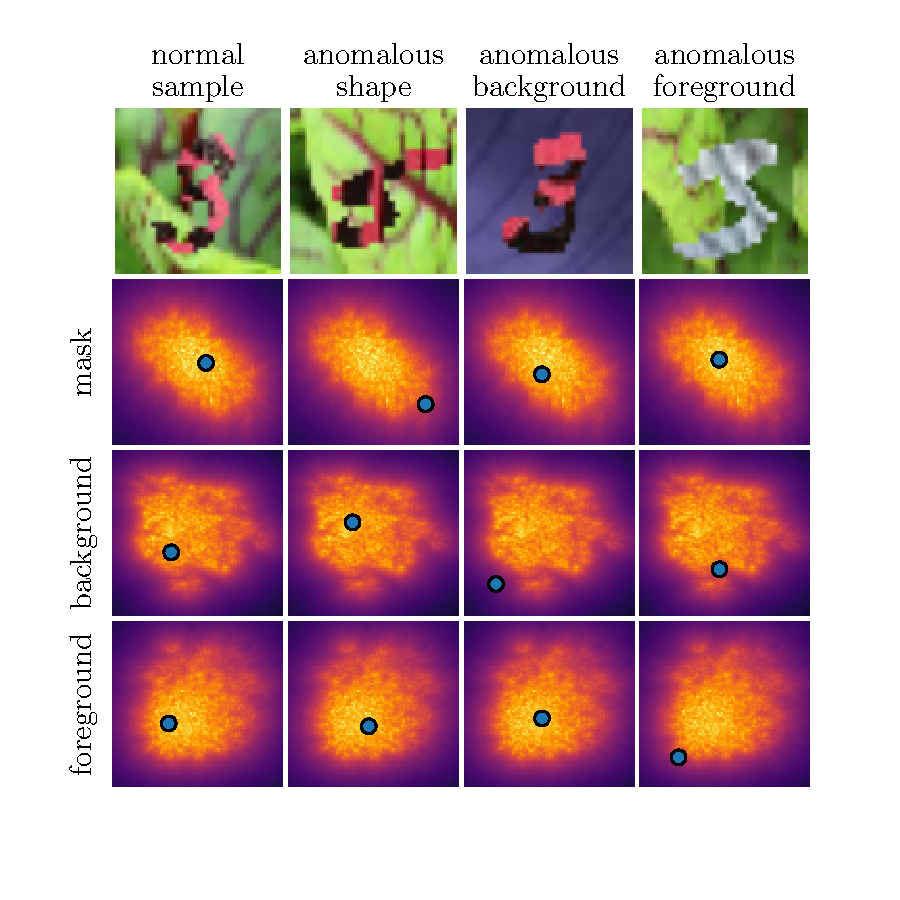
\includegraphics[width=0.95\textwidth]{data/chapter_sgvaegan/fig3_latent_decomposition_example.pdf}
    \caption{Position of different images encoded to individual latent spaces using SGVAEGAN model with two-dimensional latent spaces. The training set consisted of images with factors fixed to those of the digit in the first column. The densities of encodings of normal (training) data, estimated by a kNN detector~\eqref{eq:knnscore} are depicted as well.}
    \label{fig:latent_decomposition_example}
\end{figure}

If the SGVAEGAN is trained well, particularly if the decomposition into latent spaces is (at least approximately) right, different types of anomalies should be in low-density regions of different latent spaces. This is illustrated in Fig.~\ref{fig:latent_decomposition_example} on the Wildlife MNIST dataset, where we can see that anomalous shape, background texture, and foreground texture is anomalous in the corresponding latent space. We can use the score~\eqref{eq:alphadeco} and assign $p_{n_i}(\vc{z}_i) = p_{z_i}(\vc{z}_i), i \in \lbrace m,f,b \rbrace$, since the model is trained on normal data. Then we have
\begin{equation}
s(\vc{x}) = - \log p(\vc{e})  - \log\left\vert \frac{\partial g^{-1}(\vc{x})}{\partial \vc{x}}\right\vert -  \sum_{i\in\{m,f,b\}}\alpha_{i}\log p_{z_{i}}(\vc{z}_{i}),  
\label{eq:scorewithx}
\end{equation}
where $g(\vc{z})$ is a function that computes an image from the latent encodings via~\eqref{eq:composition}
\begin{equation}
g(\vc{z}) = g(\vc{z}_m, \vc{z}_f, \vc{z}_b) = g_{m, \vc{\theta}}(\vc{z}_m) \odot g_{f, \vc{\theta}}(\vc{z}_f) + (1 - g_{m, \vc{\theta}}(\vc{z}_m)) \odot g_{b, \vc{\theta}}(\vc{z}_b).
\end{equation}
Following the derivations in~\cite{vsmidl2019anomaly}, we use the fact that $\frac{\partial g^{-1}(\vc{x})}{\partial \vc{x}} = \left( \frac{\partial g(\vc{z})}{\partial z} \right) ^{-1}$, and assume the independency of the latent spaces of $\vc{z}_m, \vc{z}_f, \vc{z}_b$. Then Eq.~\eqref{eq:scorewithx} can be rewritten to 
\begin{align} \label{eq:scorejacodeco}  
s(\vc{x}) & = - \log p(e)  + s_j(\vc{x}) -  \sum_{i\in\{m,f,b\}} \alpha_{i}\log p_{z_{i}}(\vc{z}_{i}),
\end{align}
where $s_j(\vc{x}) = \log \left\vert  \frac{\partial g(\vc{z})}{\partial \vc{z}}  \right\vert $ denotes the Jacobian term, which is functionally dependent on the input image $\vc{x}$ through the latent encodings $\vc{z} = (\vc{z}_m, \vc{z}_f, \vc{z}_b)$, see~\eqref{eq:encoder}. A reader recognizes that $\frac{\partial g(\vc{z})}{\partial \vc{z}}$ is not square, hence its determinant is zero. Ref.~\cite{vsmidl2019anomaly} suggests estimating the determinant from a diagonal matrix after SVD decomposition, which is valid if one assumes the orthogonality of the data and noise.

The proposed score, based on~\eqref{eq:scorejacodeco}, reads as a weighted sum of the individual components
\begin{equation} \label{eq:totalscorejacobian}
    s(\vc{x}) = \alpha_{r}  s_{r}(\vc{x}) + \alpha_j s_j(\vc{x}) + \alpha_m s_{m}(\vc{x}) + \alpha_f s_{f}(\vc{x}) + \alpha_b s_{b}(\vc{x}),
\end{equation}
where $s_i, i \in \{r, j, m, f, b\}$ are individual anomaly score components which will be described in the following text. The $\alpha_r, \alpha_j$ weights were added in order to tune the total score to the modalities of anomalous data, which were not seen during the training, and therefore the base model is not fitted to them. The values of $\alpha$ can be either set manually or estimated from a small number of labeled anomalies as described in the following text.

\paragraph{Reconstruction error}
Reconstructed samples are needed for the computation of the reconstruction term $-\log p(\vc{e})$. However, since the reconstruction steps~\eqref{eq:encoder}-\eqref{eq:composition} contain sampling through the reparametrization trick, the reconstructions $\vc{x}'$ are stochastic. As we have shown already in~\eqref{eq:score_sample}, the estimate of the reconstruction error is stabilized by taking an average from multiple reconstructions $\lbrace \vc{x}'_l \rbrace_{l=1}^L$ computed as
\begin{equation} \label{eq:rsscore}
    s_{\text{r}}(\vc{x}) = - \frac{1}{\vc{\sigma}^2 L}\sum_{l=1}^L \vert \vert \vc{x}-\vc{x}'_l\vert \vert_2^2,
\end{equation}
where the scalar variance $\vc{\sigma}^2 \in \mathbb{R}$ is estimated from the data during the training of the model. The number of samples was set to $L=10$ during our experiments. 

\paragraph{Latent scores} A correct estimate of the likelihood of latent representations $p_{z_{i}}(\vc{z}_i),$ $i \in \{m, f, b\}$ is important for the score~\eqref{eq:totalscorejacobian}. Even though latent representations are regularized during the fitting of the model to have normal distribution $\mathcal{N}(0,\textbf{I})$, it was shown~\cite{dai2019diagnosing} that the fit is usually not very good. This can be also seen in Fig.~\ref{fig:latent_decomposition_example}, where the distribution of the latent representations is not perfectly normal. Therefore, we approximate $p_{z_{i}}(\vc{z}_i)$ by the k-nearest-neighbor (kNN) density estimator, see Sec.~\ref{sec:distance_methods}, which is trained on latent representations of normal data. This method was chosen for its simplicity yet powerful performance, which was demonstrated both by the results in Sec.~\ref{sec:alfven} and also in Chapter~\ref{sec:chapter_comparison}, where it scored amongst the top models on low dimensional data. This requirement will be satisfied here, as the encoders comprise the high-dimensional image data into latent space with dimensionality on the order of 10$^2$. The score of a sample in the $i$-th latent space, $i \in \lbrace m, f, b \rbrace$, has the form
\begin{equation} \label{eq:knnscore}
    s_{i}(\vc{x}) = \frac{1}{k} \sum_{\vc{z}_j \in \mathcal{Z}_{k,i}} \vert \vert \vc{z}_i - \vc{z}_j \vert \vert_2, \vc{z}_i = \vc{\mu}_{i,\vc{\phi}}(\vc{x}), 
\end{equation}
which is the average Euclidean distance between the projection $\vc{z}_i$ of the tested sample $\vc{x}$ into the latent space, and the set $\mathcal{Z}_{k,i}$ of the $k$-nearest projections of the normal data to the same latent space. The value of $k$ is a hyperparameter tuned on the validation set.

\paragraph{Optimization of $\alpha$ } The proposed score is effectively a weighted sum of individual parts. In theory, one can set the weights $\alpha$ by themselves if one knows in which latent to expect the anomaly. Since this knowledge is rarely available, we estimate them from data (that contains examples of labeled anomalies) by regularized logistic regression as
\begin{equation} \label{eq:alpha_regression}
    \alpha^* = \arg \min_{\alpha} - \sum_n y_n \log \vc{\sigma} (s(\vc{x}_n\vert\alpha)) + (1-y_n) \log(1-\vc{\sigma} (s(\vc{x}_n\vert\alpha)))) + \beta \vert \vert \alpha - \alpha_0 \vert \vert^2_2 ,
\end{equation}
\begin{equation}
    s(\vc{x}_n\vert\alpha) = \sum_i \alpha_i \hat{s}_i(\vc{x}_n), i \in \lbrace r, j, m, f, b \rbrace,
\end{equation}
where $\vc{\sigma}(.)$ is the sigmoid function, $y_n \in \lbrace 0,1 \rbrace$ are labels, $\alpha_0$ is a prior value and the index $n$ goes over the samples in the labeled dataset. Since the scores $s_i(\vc{x})$ can have very different scales (e.g. $s_r(\vc{x}) \sim 10^4$ while $s_f(\vc{x}) \sim 10^0$), we rescale them to have zero mean and unit variance. The rescaled scores are denoted as $\hat{s}_i(\vc{x})$. The regularization is set using $\beta = \frac{\beta_0}{n_1}, \beta_0 \in \mathbb{R}$, where $n_1$ is the number of positive (anomalous) samples in the dataset, and $\beta_0$ is a hyperparameter. This ensures that the prior $\alpha_0$ has a large influence over the final value of $\alpha$ when there is a small number of known anomalies, thus ensuring the robustness of the final $\alpha$ estimate. The prior is set such that $\alpha_{0,i}=1$ for such $i$ where the AUC computed from $\lbrace s_{i}(\vc{x}_n), y_n \rbrace_n$ is maximal and zero everywhere else, making $\alpha_0$ a failsafe value. The criterion~\eqref{eq:alpha_regression} is optimized by an LBFGS optimizer~\cite{liu1989limited}.

\paragraph{Removing the Jacobian from the score} 
While the score~\eqref{eq:scorejacodeco} is theoretically correct under the assumption that anomalies are located in areas of low density, the publication~\cite{vsmidl2019anomaly} shows that it does not work well when the model is trained on data without anomalies. Our experiments shown below arrived at the same conclusion. We suspect the cause to be that the decoders $g$ can be arbitrary (with arbitrary jacobian) in parts of the space not supported by the data, where anomalous samples are located. Moreover, the computation of the determinant is so expensive that the score is effectively useless for state-of-the-art image models. Therefore, we propose dropping the Jacobian term $s_j(\vc{x})$ from~\eqref{eq:totalscorejacobian} and adding the discriminator score
\begin{equation} \label{eq:discscore}
    s_d(\vc{x}) = 1 - d_{\vc{\varphi}}(\vc{x}),
\end{equation}
which works well for anomaly detection according to~\cite{larsen2016autoencoding} and also for semantic anomaly detection in images, which was shown by an exceptional performance of the fmGAN model with the score~\eqref{eq:discscore} in Chapter~\ref{sec:chapter_comparison}. The alternative score then reads
\begin{equation} \label{eq:totalscoredisc}
    s(\vc{x}) = \alpha_{r}  s_{r}(\vc{x}) + \alpha_d s_d(\vc{x}) + \alpha_m s_{m}(\vc{x}) + \alpha_f s_{f}(\vc{x}) + \alpha_b s_{b}(\vc{x}).
\end{equation}
Again, the values of $\alpha$ are optimized similarly to~\eqref{eq:alpha_regression}.

\subsection{Anomaly factor identification}
\label{sec:anomaly_factor_identification}
The model presented above can identify the source of the anomality through the information from the individual latent spaces. Under the formalism~\eqref{eq:pzy}, estimation of the probability of being generated from the normal model is simply $p(y \vert \vc{z})\propto p(\vc{z} \vert y)$, which is only possible for proper distributions. Since we used an improper distribution ($p_a(\vc{x})\propto 1$) to minimize the number of unknown parameters, we cannot use direct estimation and have to rely on approximation. This approximation relies on the fact that the source of anomaly should have a low probability in the respective latent space. We have designed two approximate methods for identifying it. The main benefit of these methods is that they are completely unsupervised and computationally cheap. Note that when using them, it is assumed that anomalies are generated from a single source, i.e. being anomalous only either in shape, foreground, or background. 

\paragraph{Ranked anomaly factor identification}
The first approximation relies on the replacement of the likelihood $p(y_i\vert \vc{z}_i(\vc{x}))$ by an empirical quantile.  Specifically, we store the values of anomaly scores $s_{i,train}=s_i(\vc{x}_{train})$ for the training set and for a new sample $\vc{x}$ compute the quantile $q_i(\vc{x})$ (relative rank) within the training scores of the corresponding latent space. The anomaly source estimate is then computed as the maximum of the relative rank $y^* = \arg\max_{i\in\{m,f,b\}}q_i(\vc{x})$.

\begin{figure}
    \centering
    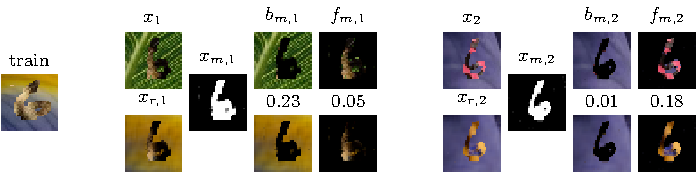
\includegraphics[width=0.95\textwidth]{data/chapter_sgvaegan/fig4_masked_examples.pdf}
    \caption{Masked detection technique for identifying the source of anomality. The model was originally trained on samples similar to the one on the very left, brown-striped sixes on a purple-yellow background. To distinguish between anomalies in the background and foreground texture, a reconstruction $\vc{x}_r$ and a mask $\vc{x}_m$ are computed for a test sample $\vc{x}_1$, which is anomalous in the background, and $\vc{x}_2$, which is anomalous in the foreground texture. The scores $S_b$ \eqref{eq:sb}, $S_f$ \eqref{eq:sf} are computed as scaled differences between the original and reconstructed masked--out backgrounds, $b_m = \vc{x} \odot (1-\vc{x}_m)$ and foregrounds $f_m = \vc{x} \odot \vc{x}_m$ and their values are displayed between the image of the original and reconstructed foregrounds and backgrounds.}
    \label{fig:masked_detection}
\end{figure}

\paragraph{Masked anomaly factor identification}
Using even a properly trained model, the ranked method is not always able to correctly identify all three types of anomaly sources. Therefore, we have simplified the problem to distinguish the source of an anomaly only in the background or foreground texture by computing the reconstruction errors for those components separately. For an input $\vc{x}$, the reconstructed image $\vc{x}'$ and a mask $\vc{x}_m$ are computed. Using these, we compute the normalized reconstruction errors as
\begin{align}
    S_b & = \frac{\sum_j \left( (\vc{x}_j-\vc{x}_{j}') (1-\vc{x}_{m,j}) \right) ^ 2}{\sum_j 1-\vc{x}_{m,j}} \label{eq:sb} \\
    S_f & = \frac{\sum_j \left( (\vc{x}_j-\vc{x}_{j}') \vc{x}_{m,j} \right) ^ 2}{\sum_j \vc{x}_{m,j}}  \label{eq:sf}
\end{align}
where index $j$ goes over elements in all dimensions of an array $\vc{x} \in \mathbb{R}^{H \times W \times 3}$ representing an RGB image. See Fig.~\ref{fig:masked_detection} for an illustration of the principle of this method. The normalization factor in (\ref{eq:sb},\ref{eq:sf}) is important since the object in the foreground usually covers fewer pixels than the background. If $S_b$ is higher, the prediction for the anomaly factor is "background" and vice versa. The comparison of the ranked and masked method is presented in Sec.~\ref{sec:anomaly_factor_identification_experiments}

%%%%%%%%%%%%%%%%%%%%%%%%%%%%%
% Experiments

\section{Experiments} \label{sec:experiments}

In the experimental evaluation of the proposed model, we follow the strict protocol that was established in Chapter~\ref{sec:chapter_comparison}. The datasets were split into training, validation, and test subsets for each of their classes (or subproblems in the case of the MVTec-AD dataset). Details on the splits for individual experiments can be found in the respective sections below. Then, for each such split and each model, 50 hyperparameter settings were randomly sampled from a set of possible values. The use of Bayesian optimization to select hyperparameters was considered but eventually dropped as it did not have an impact on the relative rank of the methods in Chapter~\ref{sec:chapter_comparison}. The validation set was used to select the best hyperparameter values for a given model on a specific subproblem. Unless mentioned otherwise, the experiments below report (ROC)AUC values of the selected models computed on the test set. The models were trained for 50 epochs each.

The datasets used in the experimental evaluation were selected in order to contain semantic anomalies (with the exception of the MVTec-AD dataset). Two artificial datasets (Wildlife MNIST and COCOPlaces) were created as baselines on which the model is supposed to perform well. Especially Wildlife MNIST contains easily segmentable objects. For details on datasets, see Appendix~\ref{sec:appendix_datasets}.

\subsection{Baseline methods}
We have selected unsupervised anomaly detectors mainly based on the review in Chapter~\ref{sec:chapter_comparison}, specifically those that were amongst the top performers on colored images. For additional These models include:

\begin{description}
    \item[\textbf{Variational Autoencoder (VAE)}] - a convolutional VAE from Sec.~\ref{sec:vae_models} that uses the sampled reconstruction error~\eqref{eq:rsscore}. The decoder variance $\vc{\sigma}^2$ is estimated from the data.
    \item[\textbf{Feature-matching GAN (fmGAN)}] - a convolutional GAN model trained using the feature-matching loss~\eqref{eq:fmgan}. The anomaly score is based on the discriminator~\eqref{eq:discscore}.
    \item[\textbf{VAEGAN}] - a  convolutional VAE where reconstruction is enforced through a discriminator~\cite{larsen2016autoencoding}. The anomaly score is~\eqref{eq:discscore}.
    \item[\textbf{Deep Support Vector Data Description (DSVDD)}] - is a model that learns a transformation of data via a neural network to a subspace where the anomalies lie outside of a hypersphere composed of transformed normal data. The anomaly score is then the distance of a point from the center of the hypersphere, see Sec.~\ref{ref:sec_deep_domain}.
    \item[\textbf{fast Anomaly GAN (fAnoGAN)}] - a GAN model trained via Wasserstein loss and gradient penalization that identifies anomalies by backward-searching the latent code $z$ that is the most likely to generate the given test samples, see Sec.~\ref{sec:gan_survey}.
    \item[\textbf{Counterfactual Generative Network (CGN)}] - this is a baseline model~\cite{sauer2021counterfactual} for the decomposition of data into three components. Although not originally intended as an anomaly detector, it can be used as one as it provides the discriminator score~\eqref{eq:discscore} and proved itself to be competitive in our experiments.
    \item[\textbf{Shape Guided VAE (SGVAE)}] - this is a modification of the proposed model introduced to study the impact of the discriminator. It is trained without a discriminator and the reconstruction loss is $ -\mathbb{E}_{q_{\vc{\phi}}(\vc{z} \vert \vc{x})}[\log p_{\vc{\theta}}(\vc{x} \vert \vc{z})]$, similar to a classical VAE. The anomaly score for this model is the sampled reconstruction error~\eqref{eq:rsscore}.
    \item[\textbf{Shape Guided VAEGAN (SGVAEGAN)}] - this is the basic proposed model that is trained in a completely unsupervised fashion and evaluated without considering the full anomaly scores~\eqref{eq:totalscorejacobian} and~\eqref{eq:totalscoredisc}. Instead, the default anomaly score is~\eqref{eq:discscore}.
    \item[\textbf{SGVAE$_{\alpha}$}] - this is the SGVAE model where the score~\eqref{eq:totalscorejacobian} is considered. To compute the anomaly scores,  SGVAE models pre-trained in an unsupervised fashion were used and only the weights $\alpha$ were computed on a validation dataset.
    \item[\textbf{SGVAEGAN$_{\alpha}$}] - this is the full proposed model. As discussed in the Sec.~\ref{sec:jacobian_contribution}, it is used with the score~\eqref{eq:totalscorejacobian} with the Jacobian, but later the Jacobian is dropped and the model is used with score~\eqref{eq:totalscoredisc}.
\end{description}
    
\subsection{The contribution of the Jacobian} \label{sec:jacobian_contribution}
\begin{table}[t] 
 \center 
 \begin{tabular}{c c c c c } 
 \toprule 
  class & AUC - no $s_j(x)$ & AUC - with $s_j(x)$ & $\alpha_r$ & $\alpha_j$  \\ 
  \midrule
  0 & 0.70 $\pm $0.04 & 0.70 $\pm $0.05 & 1.00 & 0.00  \\ 
  1 & 0.82 $\pm $0.01 & 0.82 $\pm $0.02 & 1.09 & -0.03  \\ 
  2 & 0.71 $\pm $0.02 & 0.72 $\pm $0.02 & 0.93 & -0.01  \\ 
  3 & 0.64 $\pm $0.02 & 0.64 $\pm $0.02 & 0.94 & 0.01  \\ 
  4 & 0.72 $\pm $0.03 & 0.72 $\pm $0.03 & 1.00 & 0.00  \\ 
  5 & 0.67 $\pm $0.01 & 0.66 $\pm $0.01 & 0.98 & 0.00  \\ 
  6 & 0.68 $\pm $0.02 & 0.68 $\pm $0.02 & 0.60 & 0.00  \\ 
  7 & 0.73 $\pm $0.05 & 0.73 $\pm $0.05 & 1.00 & 0.00  \\ 
  8 & 0.69 $\pm $0.04 & 0.71 $\pm $0.02 & 0.98 & -0.04  \\ 
  9 & 0.63 $\pm $0.05 & 0.63 $\pm $0.04 & 0.80 & 0.00  \\ 
  \bottomrule
 \end{tabular}
 \caption{Experiment with $s_j(x)$ on a subset of the SVHN2 dataset. The mean values of  $\alpha$ weights estimated with~\eqref{eq:alpha_regression} are also presented and show that the weight of the Jacobian term is suppressed during their computation.} 
 \label{tab:jacoceco_partial_experiment} 
\end{table}
We start by demonstrating that dropping the Jacobian term from the score~\eqref{eq:totalscorejacobian} does not have a negative effect on the detection performance of the proposed model. Tab.~\ref{tab:jacoceco_partial_experiment} shows AUCs of the model that uses the score~\eqref{eq:totalscorejacobian} with and without the Jacobian term $s_j(\vc{x})$ on a subset of the SVHN2 dataset. For each normal class, training, and testing sets containing 750 normal and 150 anomalous samples were used. To obtain the presented statistic, the subsets were sampled 5 times.  The difference in performance is almost negligible but the difference in computational costs is high. Therefore, we omit the term from all further experiments, and the score~\eqref{eq:totalscoredisc} is used for the SGVAEGAN$_{\alpha}$ instead, while for SGVAE$_\alpha$, the term is dropped from~\eqref{eq:totalscorejacobian}.

\subsection{Detection of semantic anomalies} 
\begin{figure}[ht!]
    \centering
    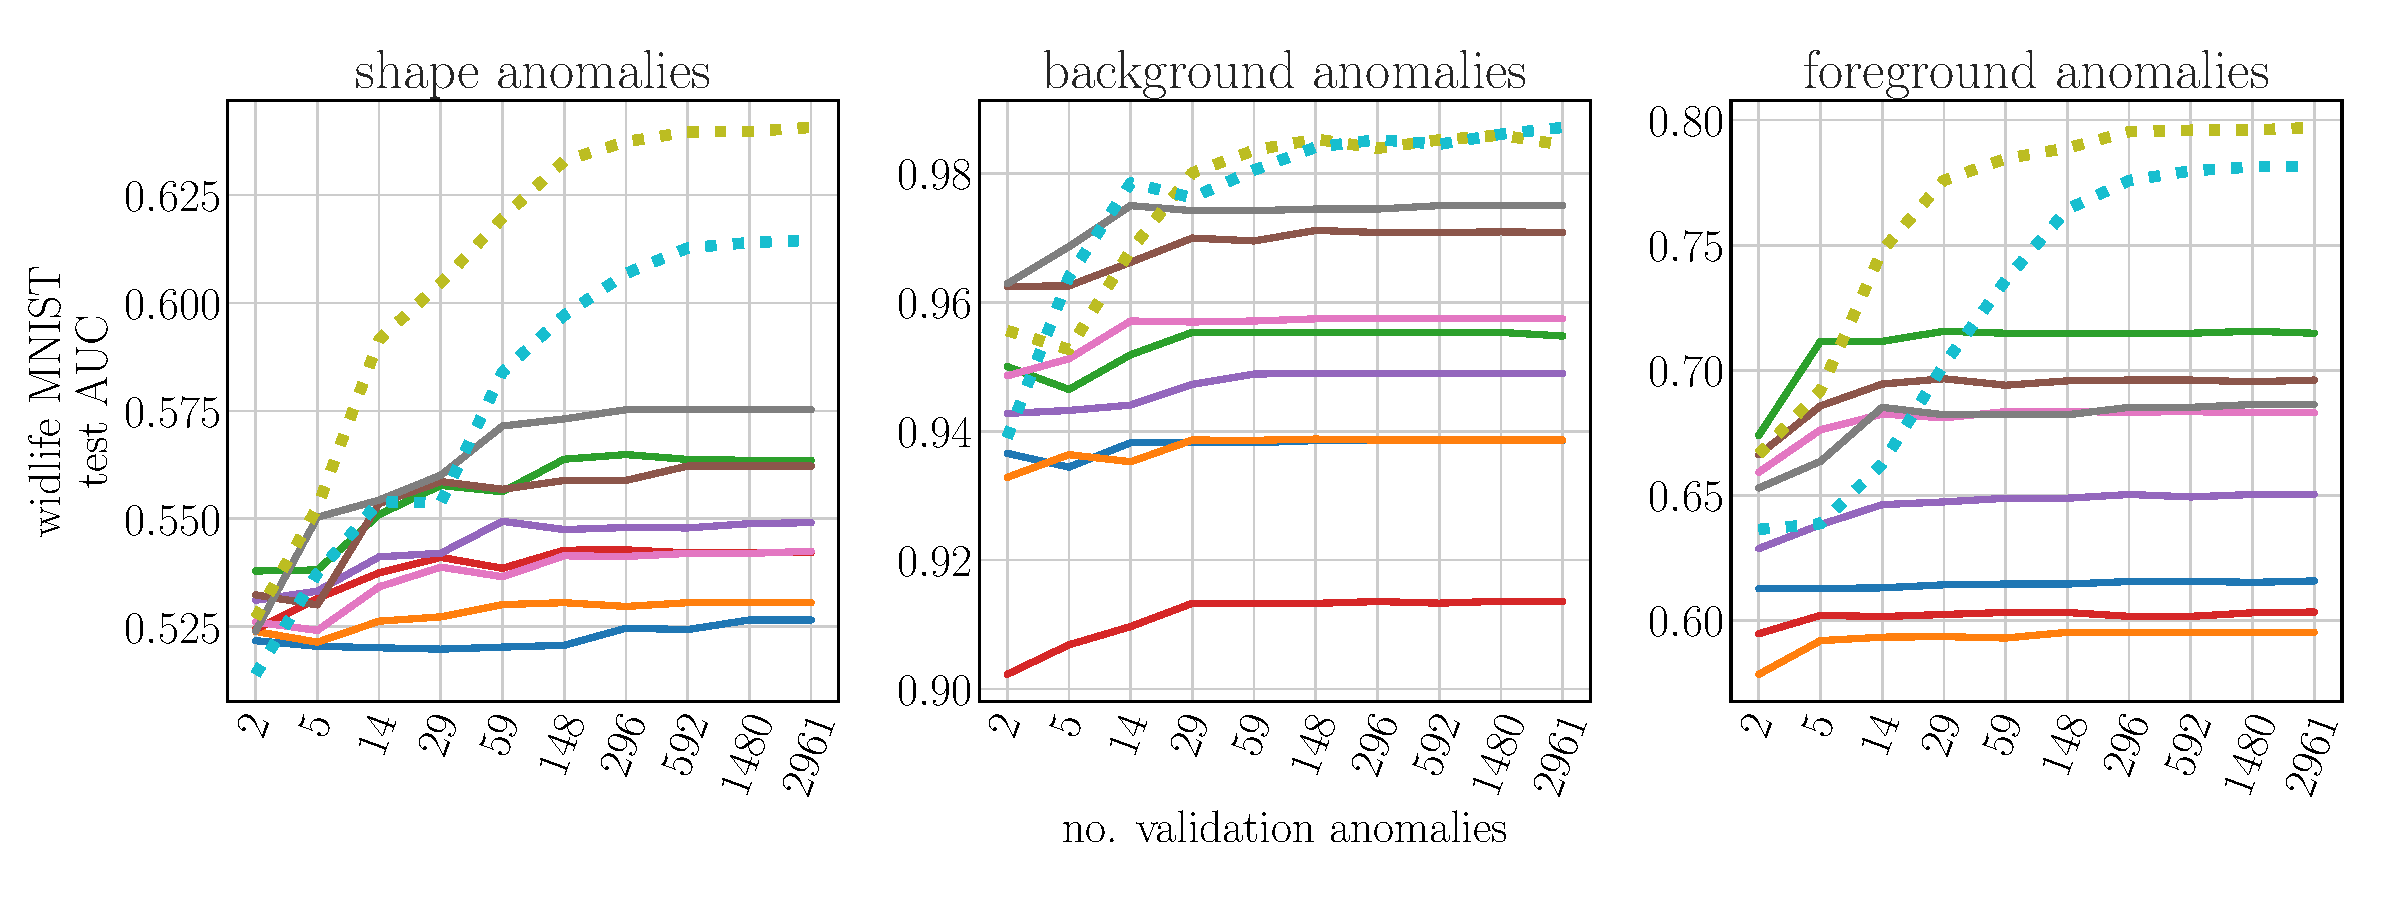
\includegraphics[width=\textwidth]{data/chapter_sgvaegan/fig6_multifactor_experiments_wmnist.pdf}
    
    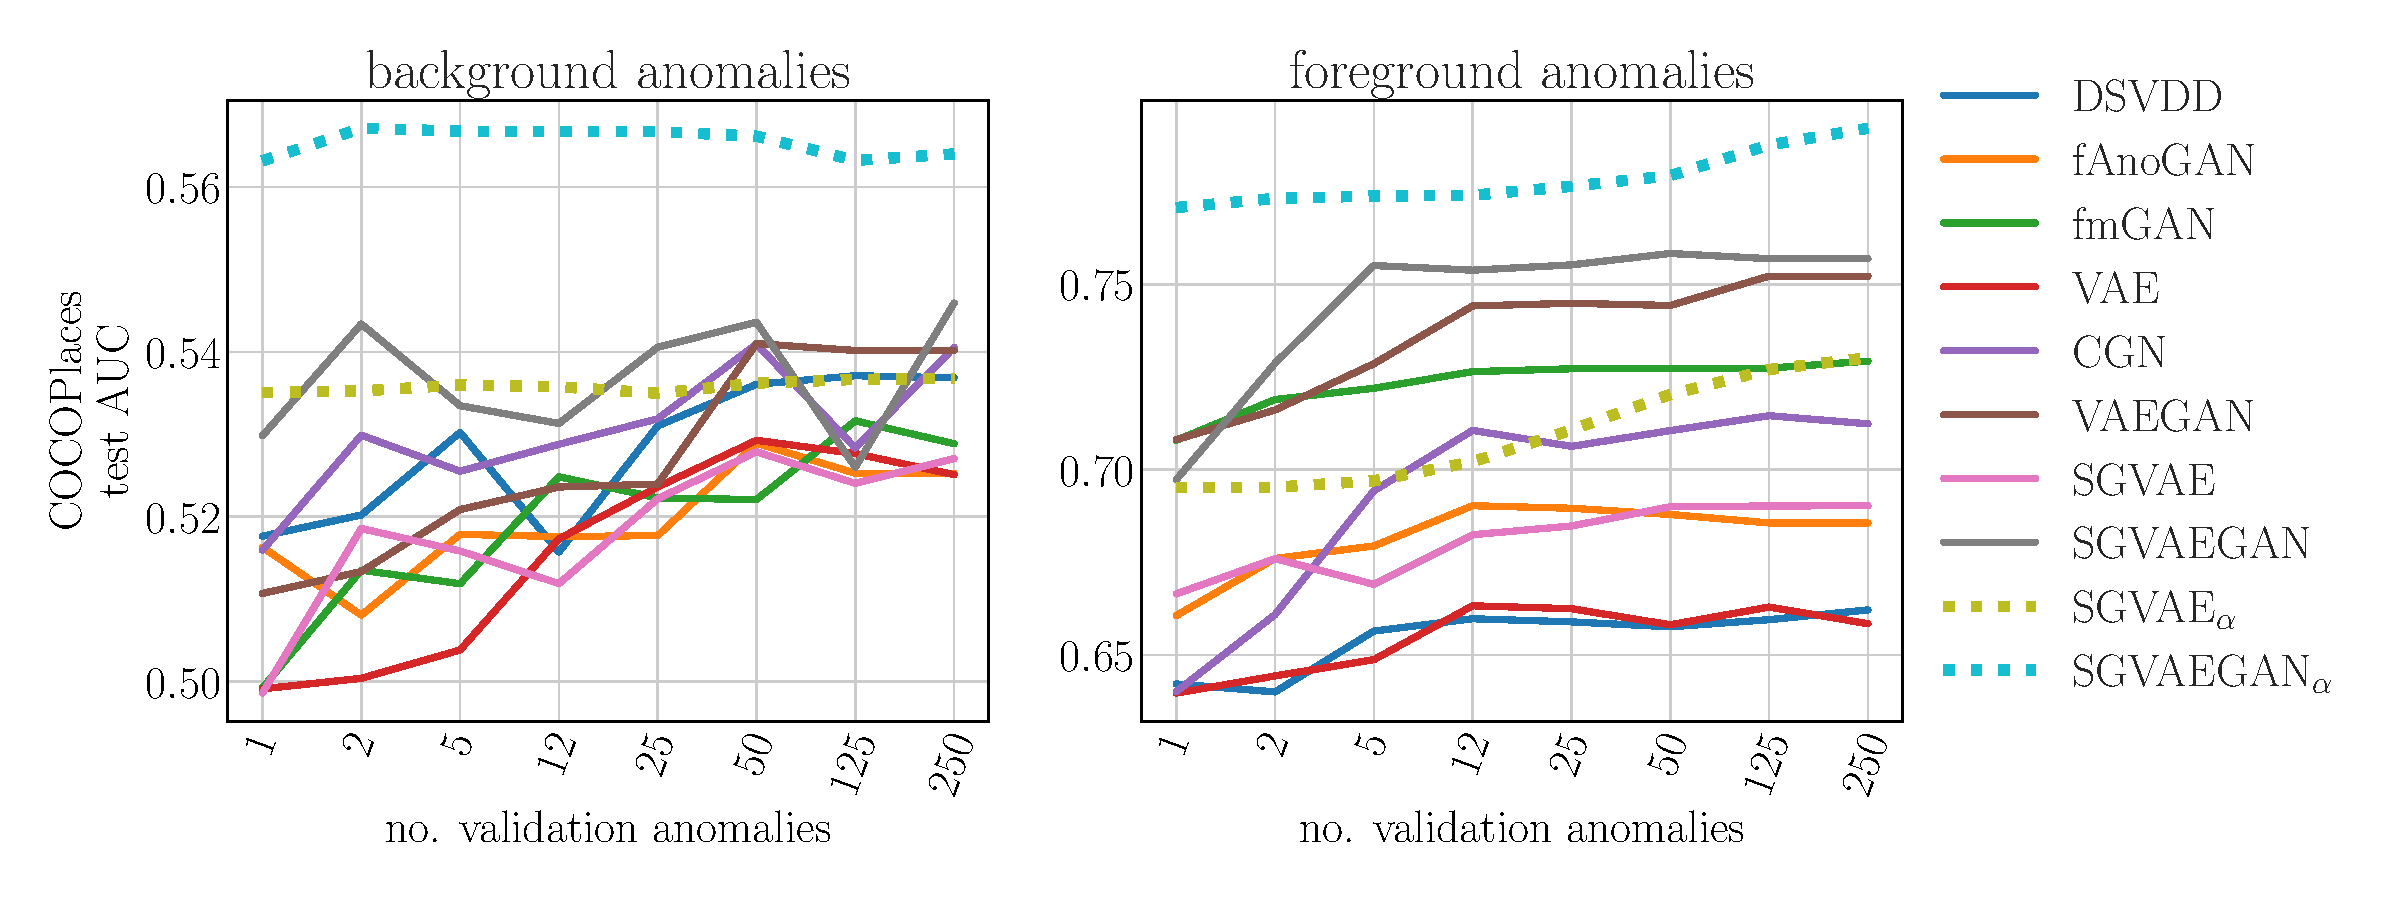
\includegraphics[width=\textwidth]{data/chapter_sgvaegan/fig7_multifactor_experiments_coco.pdf}
    \caption{Semantic anomaly detection experiment on the Wildlife MNIST (top) and COCOPlaces (bottom) datasets. The x-axis covers a changing number of anomalies present in the validation dataset. The y-axis reports the average AUC over dataset subclasses and 5-fold cross-validation.}
    \label{fig:multifactor}
\end{figure}
We now study how the proposed detector behaves as it gradually incorporates more knowledge in the form of labeled anomalies used to optimize weights $\alpha$ via~\eqref{eq:alpha_regression}. To simulate a semantic anomaly scenario, the following training and testing protocol is used with the Wildlife MNIST and COCOPlaces datasets. The training set consists of samples of one class (the whole experiment is repeated for all 10 classes) from the non-mixed version of the datasets (see Appendix.~\ref{sec:appendix_datasets} for details of how this is generated). Then, for a given factor of variation, validation, and test sets are drawn from the mixed version of the dataset, where the anomality of a sample is based on whether the target factor is the same or different as in the training dataset. This introduces a non-semantic shift, as the validation and test sets contain a variation of a factor that was not seen in the training data but is not considered anomalous. 

An example of how the individual data sets are constructed is the following: consider that the training set contains only images of MNIST class "0" with "leaf" background and brown foreground texture, like in Fig.~\ref{fig:wmnist_grid}. When the target factor of variation is \textit{background}, then in the validation and test set, all images with "leaf" background are considered normal and any other background is considered anomalous, no matter what the remaining factors of variation (digit and foreground texture) are, therefore a brown digit "0" with a blue background texture is considered anomalous, while a yellow "9" with "leaf" background is considered normal.

Fig.~\ref{fig:multifactor} shows AUCs of compared methods with respect to the number of known anomalies in the validation set, in which the ratio of anomalous to normal data ranges from 0.1\% to 100\% with the number of normal samples staying the same. The models are trained on the same training non-mixed data, their hyperparameters are selected on the validation dataset and the resulting test set AUC is averaged over 10 classes and a 5-fold random selection of the validation anomalies. While on Wildlife MNIST, both SGVAE$_\alpha$ and SGVAEGAN$_\alpha$ quickly dominate other methods once a few (five) examples of anomalies are available, the SGVAE$_\alpha$ performs worse on COCOPlaces. This is the effect of the discriminator of SGVAEGAN, which is used in the score and which contributes to the improved fit of the model. The results also show how methods benefit from a better selection of hyperparameters when more known anomalies are in the validation set.

\subsection{Anomaly factor identification} \label{sec:anomaly_factor_identification_experiments}
In this section, we compare the two approximate methods for identification of the source of an anomaly as described in Sec.~\ref{sec:anomaly_factor_identification}, i.e. the ranked and the masked method. For the comparison, we use the mixed version of the Wildlife MNIST dataset. The results in the form of prediction accuracies over different normal classes are shown in~Tab.~\ref{tab:factor_detection}. 

\begin{table}[h] 
 \center 
 \begin{tabular}{c | c c c | c c}
 \toprule
 & \multicolumn{3}{c|}{ranked} & \multicolumn{2}{c}{masked} \\
  normal class & shape & background & foreground & background & foreground  \\ 
  \midrule 
  0 & 0.82 & 0.19 & 0.62 & 0.88 & 0.95  \\ 
  1 & 0.84 & 0.92 & 0.19 & 0.85 & 1.0  \\ 
  2 & 0.92 & 0.37 & 0.7 & 0.95 & 0.6  \\  
  3 & 0.55 & 0.86 & 0.24 & 0.63 & 0.96  \\
  4 & 0.79 & 0.46 & 0.85 & 0.62 & 1.0  \\ 
  5 & 0.57 & 0.89 & 0.31 & 0.72 & 1.0  \\ 
  6 & 0.74 & 0.95 & 0.52 & 0.96 & 0.96  \\
  7 & 0.47 & 0.84 & 0.75 & 0.87 & 0.98  \\
  8 & 0.64 & 0.64 & 0.62 & 0.98 & 0.97  \\
  9 & 0.88 & 0.27 & 0.1 & 0.77 & 0.94  \\
   \bottomrule
 \end{tabular}
 \caption{Accuracy of factor detection on the wildlife MNIST dataset for \textit{ranked} and \textit{masked} methods. The columns correspond to test samples anomalous in the respective factor.} 
 \label{tab:factor_detection} 
\end{table}

The ranked method sometimes fails to identify all three factors better than random chance, which has an accuracy of 0.33. The masked method performs better than the ranked one in the identification of the background and foreground anomalies, although the background anomaly detection accuracies are not completely satisfactory on all digit classes. However, we explain this by some classes having very similar backgrounds, e.g. a very common misclassification for class "4" is that with anomalous background from classes "1" or "7", see~Fig.~\ref{fig:wmnist_grid}. In these misclassifications, the background is reconstructed rather well, while even a small imprecision in the mask leads to a high reconstruction error in the foreground. Still, this method of detection of the source of anomality might be useful in some real-world problems, given we can train the model to produce correct masks. 

\subsection{Large scale study} \label{sec:benchmarks}
\begin{figure}[ht!]
    \centering
        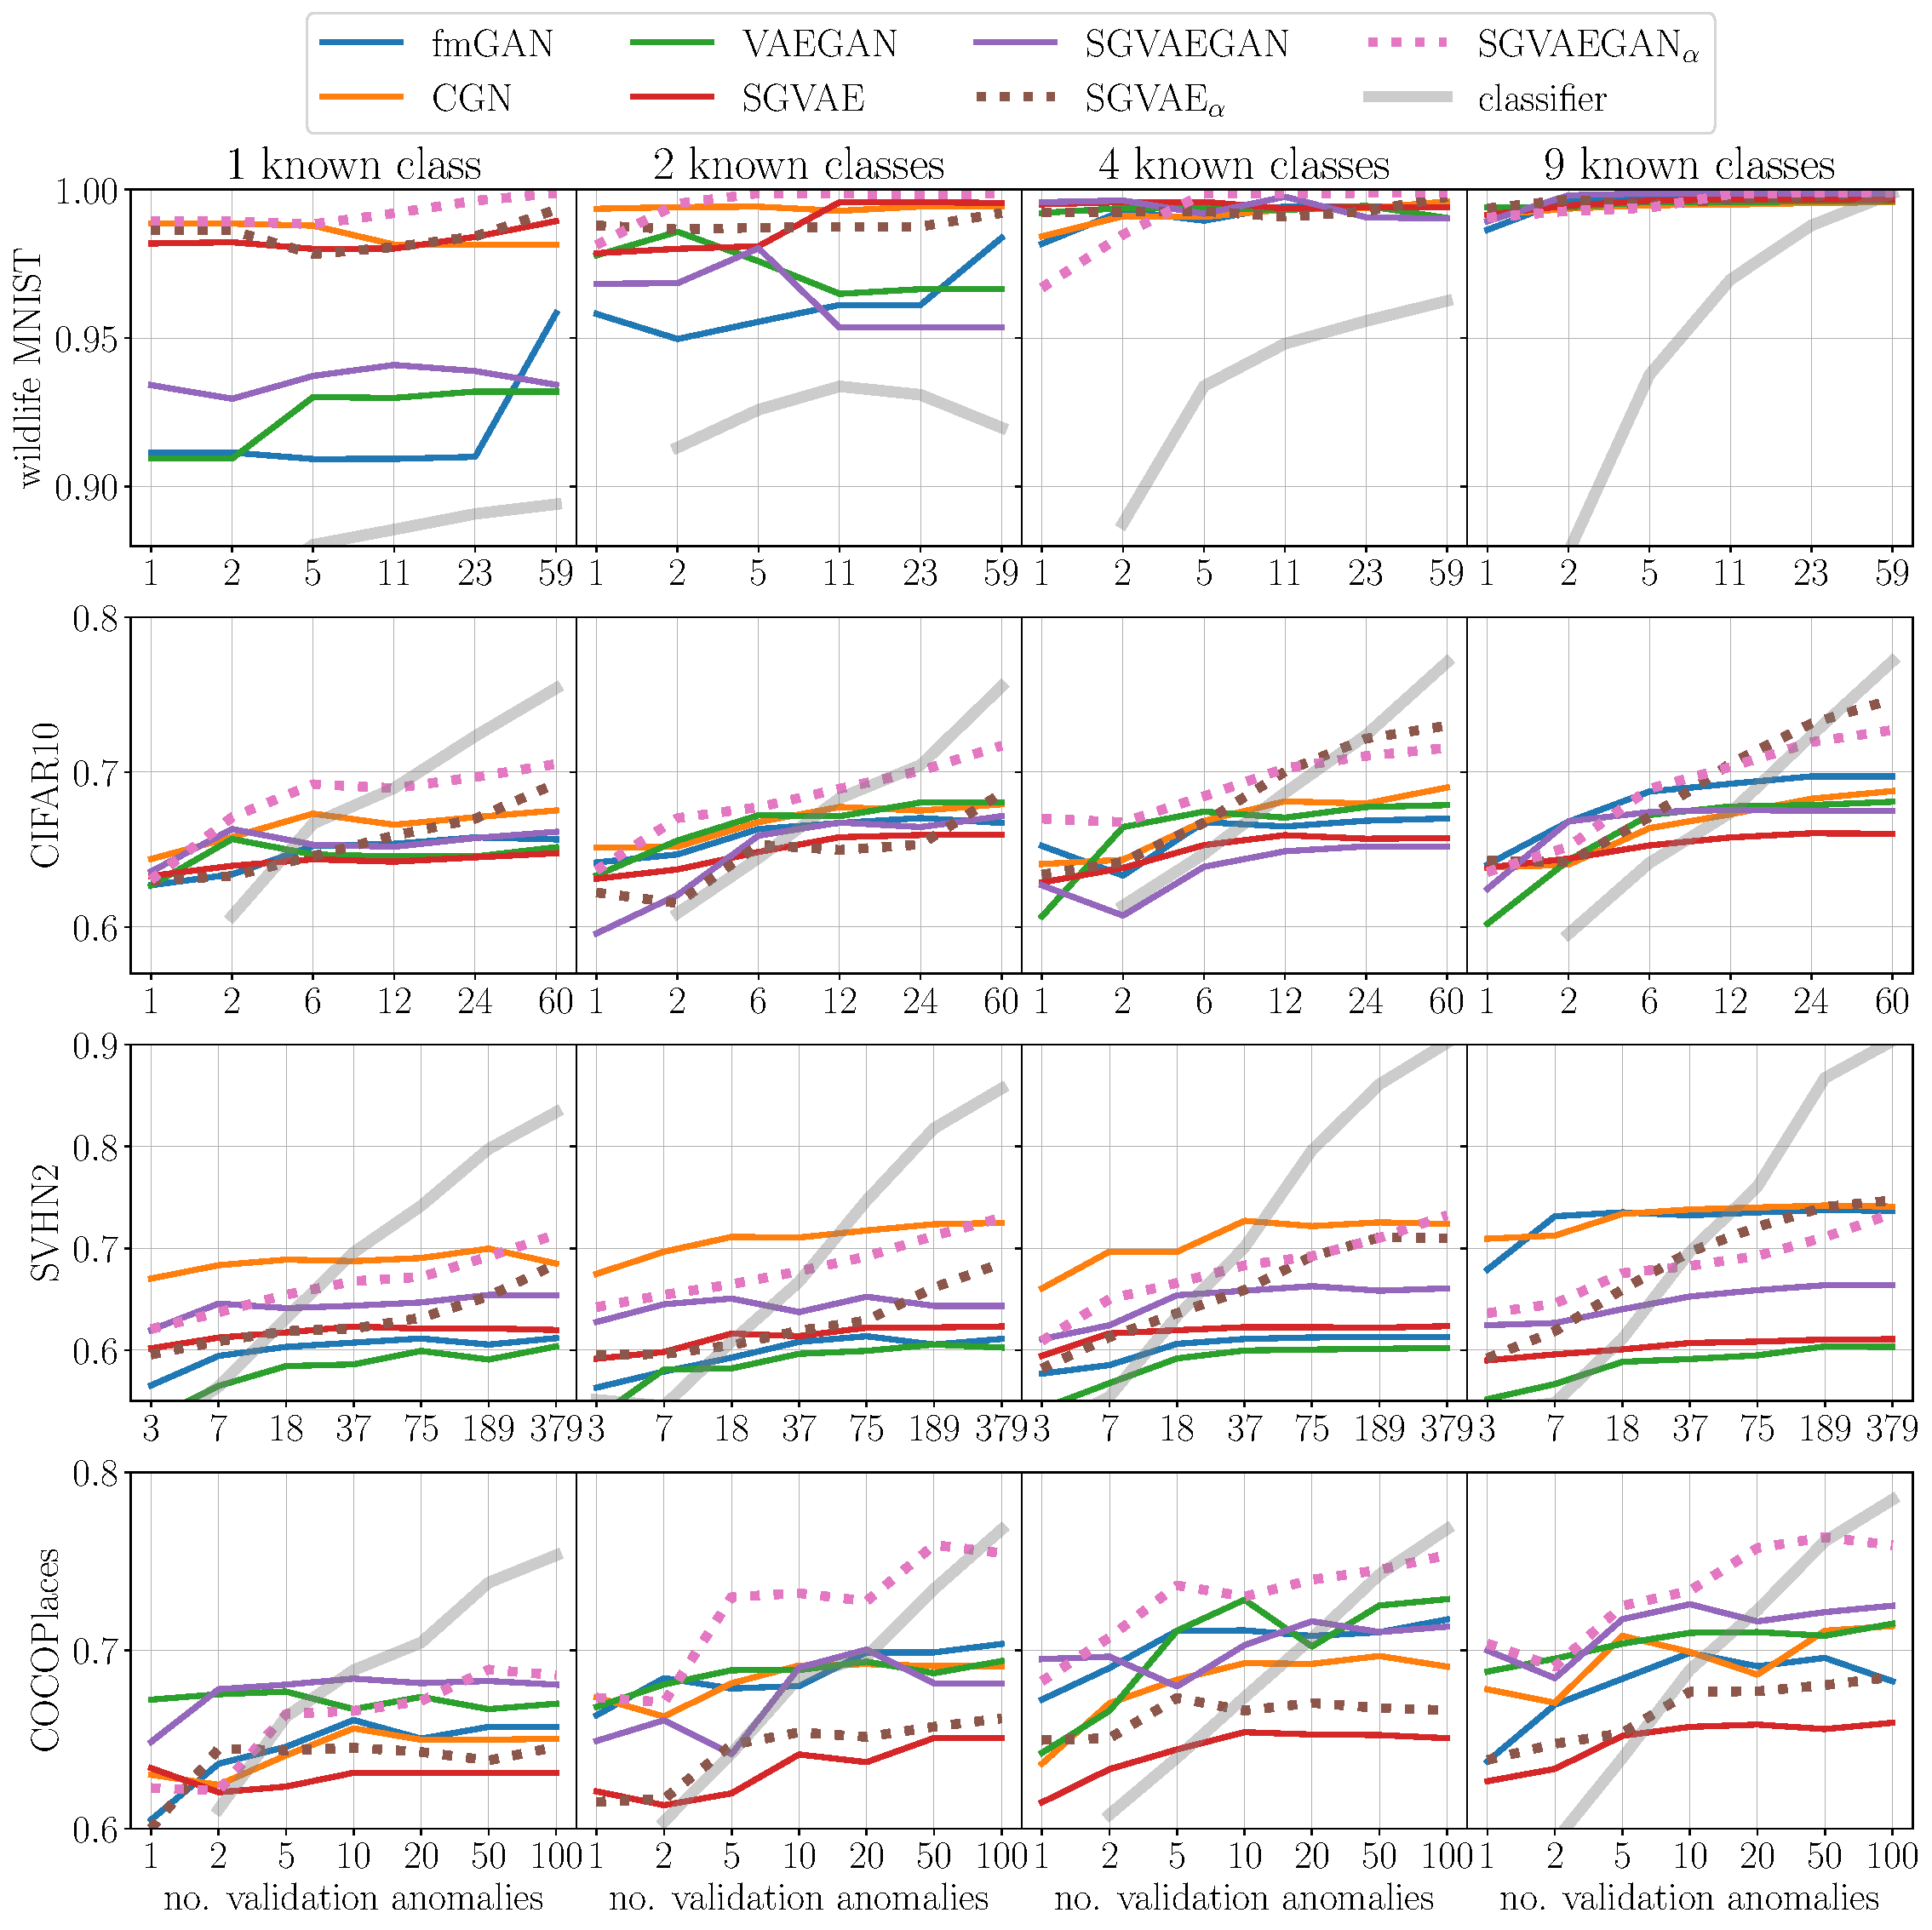
\includegraphics[width=\textwidth]{data/chapter_sgvaegan/fig8_all.pdf}
    \caption{Comparison of models on selected image datasets for the leave-one-in experiment. The x-axis covers a changing number of anomalies in the validation dataset, which is used for hyperparameter selection and $\alpha$ computation. The y-axis reports the average test AUC over 10 normal classes. The columns capture experiments with varying availability of validation samples from different anomalous classes, while anomalies of all classes are present in the test set. The number of normal samples in the validation set is the following: Wildlife MNIST: 1184, CIFAR10: 1200, SVHN2: 3792, COCOPlaces: 100.}
    \label{fig:kplots}
\end{figure}

\begin{table}[ht!] 
 \center 
 \begin{tabular}{c c c c c c c c c c c } 
  problem & \rotatebox{90}{DSVDD} & \rotatebox{90}{fAnoGAN} & \rotatebox{90}{fmGAN} & \rotatebox{90}{VAE} & \rotatebox{90}{CGN} & \rotatebox{90}{VAEGAN} & \rotatebox{90}{SGVAE} & \rotatebox{90}{SGVAEGAN} & \rotatebox{90}{SGVAE$_{\alpha}$} & \rotatebox{90}{SGVAEGAN$_{\alpha}$}  \\ 
  \midrule 
  bottle & 0.81 & \cellcolor{gray!30} 0.97 & \cellcolor{gray!15} 0.95 & \cellcolor{gray!45} 0.98 & 0.90 & 0.85 & \cellcolor{gray!45} 0.98 & 0.83 & \cellcolor{gray!30} 0.97 & 0.92  \\ 
  capsule & 0.65 & 0.69 & 0.67 & \cellcolor{gray!15} 0.74 & 0.69 & 0.58 & \cellcolor{gray!30} 0.76 & 0.66 & \cellcolor{gray!45} 0.80 & 0.67  \\ 
  nut & 0.78 & 0.72 & \cellcolor{gray!45} 0.88 & 0.71 & 0.82 & \cellcolor{gray!15} 0.84 & 0.69 & 0.78 & 0.81 & \cellcolor{gray!30} 0.86  \\ 
  pill & 0.64 & 0.71 & \cellcolor{gray!15} 0.73 & \cellcolor{gray!15} 0.73 & 0.59 & 0.70 & \cellcolor{gray!30} 0.77 & 0.72 & \cellcolor{gray!45} 0.78 & \cellcolor{gray!15} 0.73  \\ 
  transistor & 0.69 & 0.77 & \cellcolor{gray!45} 0.90 & \cellcolor{gray!15} 0.81 & \cellcolor{gray!30} 0.88 & 0.75 & 0.78 & 0.79 & \cellcolor{gray!15} 0.81 & 0.79  \\ 
  \midrule
  mean rank & 8.90 & 6.20 & \cellcolor{gray!30} 3.50 & \cellcolor{gray!15} 4.20 & 5.50 & 7.60 & 4.50 & 7.00 & \cellcolor{gray!45} 2.80 & 4.80  \\ 
  \bottomrule
 \end{tabular}
 \caption{Aggregated performance in test AUC of models on MVTec-AD problems.} 
 \label{tab:mvtec} 
\end{table}

\begin{figure}[ht!] 
    \centering
    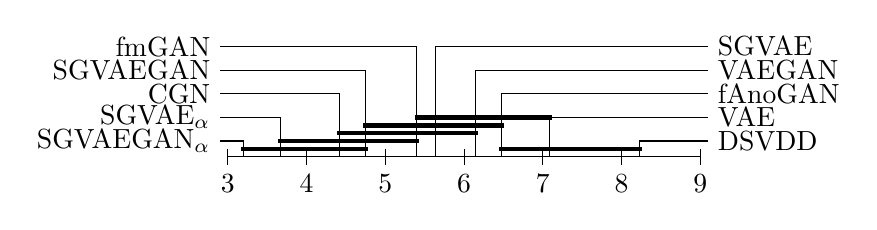
\begin{tikzpicture}[scale=1.0] 
  \draw (3.0,0) -- (9.0,0); 
  \foreach \x in {3,...,9} \draw (\x,0.10) -- (\x,-0.10) node[anchor=north]{$\x$}; 
  \draw (3.2,0) -- (3.2,0.19999999999999998) -- (2.9, 0.19999999999999998) node[anchor=east] {SGVAEGAN$_{\alpha}$}; 
  \draw (3.6625,0) -- (3.6625,0.5) -- (2.9, 0.5) node[anchor=east] {SGVAE$_{\alpha}$}; 
  \draw (4.4125,0) -- (4.4125,0.7999999999999999) -- (2.9, 0.7999999999999999) node[anchor=east] {CGN}; 
  \draw (4.75,0) -- (4.75,1.0999999999999999) -- (2.9, 1.0999999999999999) node[anchor=east] {SGVAEGAN}; 
  \draw (5.4,0) -- (5.4,1.4) -- (2.9, 1.4) node[anchor=east] {fmGAN}; 
  \draw (5.6375,0) -- (5.6375,1.4) -- (9.1, 1.4) node[anchor=west] {SGVAE}; 
  \draw (6.15,0) -- (6.15,1.0999999999999999) -- (9.1, 1.0999999999999999) node[anchor=west] {VAEGAN}; 
  \draw (6.475,0) -- (6.475,0.8) -- (9.1, 0.8) node[anchor=west] {fAnoGAN}; 
  \draw (7.0875,0) -- (7.0875,0.5) -- (9.1, 0.5) node[anchor=west] {VAE}; 
  \draw (8.225,0) -- (8.225,0.2) -- (9.1, 0.2) node[anchor=west] {DSVDD}; 
  \draw[line width=0.06cm,color=black,draw opacity=1.0] (3.170000047683716,0.1) -- (4.78,0.1); 
  \draw[line width=0.06cm,color=black,draw opacity=1.0] (3.6324999046325686,0.2) -- (5.430000095367432,0.2); 
  \draw[line width=0.06cm,color=black,draw opacity=1.0] (4.382499904632568,0.30000000000000004) -- (6.180000095367432,0.30000000000000004); 
  \draw[line width=0.06cm,color=black,draw opacity=1.0] (4.72,0.4) -- (6.504999904632569,0.4); 
  \draw[line width=0.06cm,color=black,draw opacity=1.0] (5.370000095367431,0.5) -- (7.117500095367432,0.5); 
  \draw[line width=0.06cm,color=black,draw opacity=1.0] (6.444999904632568,0.1) -- (8.255000381469726,0.1); 
 \end{tikzpicture} 

    \caption{A critical difference diagram that shows mean ranks of models from Tab.~\ref{tab:loi_ranks_per_ac}. The difference in the performance of 2 models compared on 40 datasets to be statistically significant on level 10\% must be greater than the value of the Nemenyi test $CD_{0.1}$=1.95. The thick horizontal lines connect the models with performance differences less than this.}
    \label{fig:cd}
\end{figure}

This experiment compares the proposed model in a traditional anomaly detection scenario on selected image datasets. We assume the leave-one-in scenario, when the training dataset contains samples from one class and the rest is considered to be anomalous in validation and test datasets. We believe this is a good representation of a semantic anomaly detection problem as well as being a more realistic option since in real-world problems, anomalies may come from many varying distributions.\footnote{In this regard, we disagree with the authors of~\cite{ahmed2020detecting} which propose the alternative of leave-one-out, stating that in most anomaly detection problems, we want to detect only small perturbations from the target class. However, traditional image benchmarks don't allow for this anyway as the classes are very distinct even in the latter case.} To test the models in a non-semantic anomaly detection setting, we have included the MVTec-AD dataset where the normal and anomalous data differ only in small details, and which is popular for benchmarking anomaly detection methods.

In practice, it might happen that anomalies are in a few clusters, but only samples from some of them are labeled and available for model selection. To simulate such a scenario and similar validation/test discrepancies, we performed model selection with significantly varied validation sets. First, the total number of anomalies in the validation set was varied, which constitutes the x-axis in Fig.~\ref{fig:kplots}. Second, for each normal class, samples from only a limited number of anomalous classes were sampled to the validation set, which creates the different columns in Fig.~\ref{fig:kplots}. The test set contained anomalies from all the classes left out of training. An example with 4 anomalous classes known in validation: training of models was done using class "1" of the SVHN2 dataset. The validation dataset contained normal data from class "1" and anomalies sampled from classes "2", "3", "4" and "5". The testing dataset contained normal samples from class "1" and anomalies sampled from all the other classes. The normal data split is 60/20/20\%, 50\% of available anomalies are in the test set. 

Fig.~\ref{fig:kplots} contains the overall comparison across the different variants of validation datasets used for model selection. It contains only a selection of the best-performing models to improve readability. Apart from the SVHN2 dataset, the proposed model outperforms the baselines after observing just 10 examples of anomalies, in some cases even less. A comparison of all baselines aggregated over all semantic datasets is presented in the critical difference diagram in Fig.~\ref{fig:cd}, where mean ranks of models are compared using the methodology presented in~\cite{demsar2006statistical}. Tab.~\ref{tab:loi_ranks_per_ac} contains a disaggregated comparison in the case of 2\% of labeled anomalies from 4 classes in the validation dataset. Finally, see Tab.~\ref{tab:mvtec} for the results on the MVTec-AD subproblems. Here the alternative SGVAE$_{\alpha}$ trained without a discriminator performs better. This is probably because the dataset only contains non-semantic anomalies, which cannot be well captured by the discriminator score which is used in SGVAEGAN$_{\alpha}$. Since the total number of anomalies in MVTec-AD is low, the use of the discriminator score may lead to overfitting of the $\alpha$ estimate on the validation dataset. By selecting the optimal model on the validation set and reporting on the test set, which is not standard in every publication~\cite{vskvara2021comparison}, we believe that our experiments provide a realistic comparison of baselines.

\begin{table}[ht!] 
 \center 
 \resizebox{\textwidth}{!}{ 
 \begin{tabular}{c c c c c c c c c c c c } 
  & class & \rotatebox{90}{DSVDD} & \rotatebox{90}{fAnoGAN} & \rotatebox{90}{fmGAN} & \rotatebox{90}{VAE} & \rotatebox{90}{CGN} & \rotatebox{90}{VAEGAN} & \rotatebox{90}{SGVAE} & \rotatebox{90}{SGVAEGAN} & \rotatebox{90}{SGVAE$_{\alpha}$} & \rotatebox{90}{SGVAEGAN$_{\alpha}$}  \\ 
  \toprule
  \parbox[t]{1mm}{\multirow{10}{*}{\rotatebox[origin=c]{90}{wildlife MNIST}}} & 0 & 0.82 & \cellcolor{gray!15} 0.98 & \cellcolor{gray!45} 1.00 & 0.94 & \cellcolor{gray!45} 1.00 & \cellcolor{gray!45} 1.00 & \cellcolor{gray!45} 1.00 & \cellcolor{gray!45} 1.00 & \cellcolor{gray!30} 0.99 & \cellcolor{gray!45} 1.00  \\ 
   & 1 & \cellcolor{gray!30} 0.88 & \cellcolor{gray!45} 1.00 & \cellcolor{gray!45} 1.00 & \cellcolor{gray!45} 1.00 & \cellcolor{gray!45} 1.00 & \cellcolor{gray!45} 1.00 & \cellcolor{gray!45} 1.00 & \cellcolor{gray!45} 1.00 & \cellcolor{gray!45} 1.00 & \cellcolor{gray!45} 1.00  \\ 
    & 2 & 0.63 & \cellcolor{gray!15} 0.97 & \cellcolor{gray!45} 1.00 & 0.85 & \cellcolor{gray!30} 0.99 & \cellcolor{gray!45} 1.00 & 0.96 & 0.93 & \cellcolor{gray!30} 0.99 & \cellcolor{gray!45} 1.00  \\ 
    & 3 & \cellcolor{gray!15} 0.83 & \cellcolor{gray!30} 0.99 & \cellcolor{gray!30} 0.99 & \cellcolor{gray!30} 0.99 & \cellcolor{gray!30} 0.99 & \cellcolor{gray!30} 0.99 & \cellcolor{gray!45} 1.00 & \cellcolor{gray!45} 1.00 & \cellcolor{gray!45} 1.00 & \cellcolor{gray!45} 1.00  \\ 
    & 4 & \cellcolor{gray!15} 0.91 & \cellcolor{gray!45} 1.00 & \cellcolor{gray!30} 0.99 & \cellcolor{gray!30} 0.99 & \cellcolor{gray!45} 1.00 & \cellcolor{gray!45} 1.00 & \cellcolor{gray!45} 1.00 & \cellcolor{gray!30} 0.99 & \cellcolor{gray!45} 1.00 & \cellcolor{gray!45} 1.00  \\ 
    & 5 & 0.39 & \cellcolor{gray!15} 0.93 & \cellcolor{gray!30} 0.99 & 0.85 & \cellcolor{gray!30} 0.99 & \cellcolor{gray!30} 0.99 & \cellcolor{gray!45} 1.00 & \cellcolor{gray!45} 1.00 & \cellcolor{gray!45} 1.00 & \cellcolor{gray!45} 1.00  \\ 
    & 6 & \cellcolor{gray!30} 0.69 & \cellcolor{gray!45} 1.00 & \cellcolor{gray!45} 1.00 & \cellcolor{gray!45} 1.00 & \cellcolor{gray!45} 1.00 & \cellcolor{gray!45} 1.00 & \cellcolor{gray!45} 1.00 & \cellcolor{gray!45} 1.00 & \cellcolor{gray!45} 1.00 & \cellcolor{gray!45} 1.00  \\ 
    & 7 & 0.92 & \cellcolor{gray!30} 0.99 & \cellcolor{gray!30} 0.99 & \cellcolor{gray!45} 1.00 & \cellcolor{gray!30} 0.99 & \cellcolor{gray!30} 0.99 & \cellcolor{gray!45} 1.00 & \cellcolor{gray!45} 1.00 & \cellcolor{gray!45} 1.00 & \cellcolor{gray!15} 0.97  \\ 
    & 8 & \cellcolor{gray!45} 1.00 & \cellcolor{gray!45} 1.00 & \cellcolor{gray!45} 1.00 & \cellcolor{gray!45} 1.00 & \cellcolor{gray!45} 1.00 & \cellcolor{gray!45} 1.00 & \cellcolor{gray!45} 1.00 & \cellcolor{gray!45} 1.00 & \cellcolor{gray!45} 1.00 & \cellcolor{gray!45} 1.00  \\ 
    & 9 & 0.71 & \cellcolor{gray!15} 0.94 & \cellcolor{gray!30} 0.99 & \cellcolor{gray!15} 0.94 & \cellcolor{gray!30} 0.99 & \cellcolor{gray!45} 1.00 & \cellcolor{gray!30} 0.99 & \cellcolor{gray!45} 1.00 & \cellcolor{gray!30} 0.99 & \cellcolor{gray!45} 1.00  \\ 
  \midrule
    \parbox[t]{1mm}{\multirow{10}{*}{\rotatebox[origin=c]{90}{CIFAR10}}} & airplane & 0.72 & 0.72 & 0.68 & 0.68 & 0.68 & \cellcolor{gray!15} 0.78 & \cellcolor{gray!15} 0.78 & 0.76 & \cellcolor{gray!30} 0.81 & \cellcolor{gray!45} 0.87  \\ 
    & automobile & 0.63 & 0.56 & 0.69 & 0.62 & \cellcolor{gray!45} 0.78 & \cellcolor{gray!15} 0.75 & 0.46 & \cellcolor{gray!30} 0.76 & 0.74 & \cellcolor{gray!45} 0.78  \\ 
    & bird & 0.67 & 0.67 & 0.60 & 0.66 & 0.60 & 0.56 & \cellcolor{gray!30} 0.70 & 0.47 & \cellcolor{gray!15} 0.68 & \cellcolor{gray!45} 0.72  \\ 
    & cat & 0.61 & 0.58 & 0.59 & 0.57 & \cellcolor{gray!15} 0.62 & 0.60 & 0.59 & 0.56 & \cellcolor{gray!45} 0.69 & \cellcolor{gray!30} 0.65  \\ 
    & deer & 0.71 & \cellcolor{gray!15} 0.75 & 0.65 & 0.74 & 0.66 & 0.63 & 0.74 & 0.66 & \cellcolor{gray!45} 0.78 & \cellcolor{gray!30} 0.77  \\ 
    & dog & 0.60 & 0.59 & \cellcolor{gray!15} 0.65 & 0.58 & 0.64 & 0.64 & 0.59 & 0.63 & \cellcolor{gray!30} 0.67 & \cellcolor{gray!45} 0.69  \\ 
    & frog & 0.71 & \cellcolor{gray!15} 0.76 & 0.71 & 0.75 & 0.67 & 0.69 & 0.73 & 0.60 & \cellcolor{gray!30} 0.78 & \cellcolor{gray!45} 0.82  \\ 
    & horse & 0.61 & 0.56 & 0.60 & 0.54 & \cellcolor{gray!45} 0.75 & \cellcolor{gray!30} 0.72 & 0.67 & 0.65 & \cellcolor{gray!15} 0.70 & 0.68  \\ 
    & ship & 0.74 & \cellcolor{gray!15} 0.80 & 0.77 & 0.71 & 0.74 & 0.71 & \cellcolor{gray!30} 0.82 & 0.72 & \cellcolor{gray!45} 0.84 & 0.79  \\ 
    & truck & 0.67 & 0.65 & \cellcolor{gray!45} 0.79 & 0.63 & \cellcolor{gray!15} 0.76 & 0.67 & 0.54 & 0.70 & 0.73 & \cellcolor{gray!30} 0.78  \\ 
    \midrule
    \parbox[t]{1mm}{\multirow{10}{*}{\rotatebox[origin=c]{90}{SVHN2}}} & 0 & 0.64 & 0.64 & 0.68 & 0.64 & \cellcolor{gray!45} 0.78 & 0.64 & 0.67 & 0.65 & \cellcolor{gray!15} 0.71 & \cellcolor{gray!30} 0.77  \\ 
    & 1 & 0.63 & 0.60 & 0.61 & 0.67 & \cellcolor{gray!15} 0.76 & 0.61 & 0.69 & 0.70 & \cellcolor{gray!30} 0.82 & \cellcolor{gray!45} 0.84  \\ 
    & 2 & 0.61 & 0.58 & 0.58 & 0.62 & \cellcolor{gray!45} 0.76 & 0.62 & 0.62 & 0.63 & \cellcolor{gray!30} 0.75 & \cellcolor{gray!15} 0.74  \\ 
    & 3 & 0.55 & 0.55 & 0.59 & 0.58 & \cellcolor{gray!45} 0.71 & 0.54 & 0.59 & \cellcolor{gray!15} 0.64 & \cellcolor{gray!15} 0.64 & \cellcolor{gray!30} 0.68  \\ 
    & 4 & 0.58 & 0.58 & 0.63 & 0.63 & \cellcolor{gray!45} 0.80 & 0.66 & 0.62 & 0.69 & \cellcolor{gray!15} 0.74 & \cellcolor{gray!30} 0.77  \\ 
    & 5 & 0.56 & 0.57 & 0.61 & 0.58 & \cellcolor{gray!45} 0.72 & 0.57 & 0.60 & 0.65 & \cellcolor{gray!15} 0.67 & \cellcolor{gray!30} 0.69  \\ 
    & 6 & 0.57 & 0.60 & 0.58 & 0.59 & \cellcolor{gray!45} 0.75 & 0.62 & 0.61 & 0.66 & \cellcolor{gray!30} 0.73 & \cellcolor{gray!15} 0.72  \\ 
    & 7 & 0.59 & 0.58 & 0.66 & 0.64 & \cellcolor{gray!45} 0.82 & 0.61 & 0.65 & 0.69 & \cellcolor{gray!15} 0.77 & \cellcolor{gray!30} 0.78  \\ 
    & 8 & 0.58 & 0.60 & 0.57 & 0.58 & \cellcolor{gray!30} 0.70 & 0.57 & 0.59 & \cellcolor{gray!15} 0.65 & \cellcolor{gray!15} 0.65 & \cellcolor{gray!45} 0.71  \\ 
    & 9 & 0.56 & 0.59 & 0.62 & 0.59 & \cellcolor{gray!45} 0.74 & 0.56 & 0.60 & 0.65 & \cellcolor{gray!15} 0.68 & \cellcolor{gray!30} 0.71  \\ 
    \midrule
    \parbox[t]{1mm}{\multirow{10}{*}{\rotatebox[origin=c]{90}{COCOPlaces}}} & airplane & 0.72 & 0.74 & \cellcolor{gray!15} 0.77 & 0.74 & 0.68 & \cellcolor{gray!30} 0.79 & 0.64 & \cellcolor{gray!45} 0.81 & \cellcolor{gray!15} 0.77 & \cellcolor{gray!45} 0.81  \\ 
    & bird & 0.48 & 0.48 & 0.64 & 0.53 & 0.64 & 0.61 & 0.47 & \cellcolor{gray!45} 0.69 & \cellcolor{gray!15} 0.66 & \cellcolor{gray!30} 0.68  \\ 
    & boat & 0.65 & 0.70 & \cellcolor{gray!45} 0.81 & \cellcolor{gray!15} 0.76 & \cellcolor{gray!15} 0.76 & \cellcolor{gray!30} 0.77 & \cellcolor{gray!30} 0.77 & 0.71 & \cellcolor{gray!30} 0.77 & \cellcolor{gray!45} 0.81  \\ 
    & bus & 0.58 & 0.82 & \cellcolor{gray!15} 0.85 & 0.67 & 0.83 & \cellcolor{gray!30} 0.87 & 0.74 & 0.70 & 0.78 & \cellcolor{gray!45} 0.89  \\ 
    & dog & \cellcolor{gray!30} 0.72 & \cellcolor{gray!15} 0.71 & \cellcolor{gray!15} 0.71 & \cellcolor{gray!30} 0.72 & 0.63 & 0.64 & \cellcolor{gray!15} 0.71 & 0.66 & \cellcolor{gray!15} 0.71 & \cellcolor{gray!45} 0.75  \\ 
    & horse & 0.58 & 0.57 & \cellcolor{gray!15} 0.69 & 0.65 & 0.59 & \cellcolor{gray!30} 0.71 & 0.65 & \cellcolor{gray!15} 0.69 & 0.64 & \cellcolor{gray!45} 0.74  \\ 
    & motorcycle & 0.63 & 0.65 & \cellcolor{gray!15} 0.75 & 0.60 & \cellcolor{gray!30} 0.77 & \cellcolor{gray!30} 0.77 & 0.69 & 0.73 & 0.66 & \cellcolor{gray!45} 0.78  \\ 
    & train & 0.64 & 0.71 & 0.68 & 0.65 & 0.55 & 0.62 & 0.69 & \cellcolor{gray!15} 0.74 & \cellcolor{gray!30} 0.75 & \cellcolor{gray!45} 0.77  \\ 
    & truck & 0.48 & 0.65 & 0.61 & 0.63 & 0.63 & \cellcolor{gray!30} 0.69 & 0.63 & \cellcolor{gray!45} 0.70 & \cellcolor{gray!15} 0.68 & 0.64  \\ 
    & zebra & 0.68 & 0.63 & 0.59 & 0.66 & \cellcolor{gray!30} 0.84 & \cellcolor{gray!15} 0.82 & 0.52 & 0.79 & \cellcolor{gray!45} 0.86 & \cellcolor{gray!30} 0.84  \\ 
  \midrule
  & mean rank & 8.23 & 6.48 & 5.40 & 7.09 & \cellcolor{gray!15} 4.41 & 6.15 & 5.64 & 4.75 & \cellcolor{gray!30} 3.66 & \cellcolor{gray!45} 3.20  \\ 
  \bottomrule
 \end{tabular}
 }
 \caption{Test AUC of models trained on the normal class marked in the first column of the table. The shading highlights the top 3 models. In this experiment, the validation dataset contained anomalies from 4 known classes, which is the same as the third column in Fig.~\ref{fig:kplots}. The ratio of normal data and anomalies in the validation dataset was 100:2. In absolute numbers, this means the following numbers of validation anomalies: wildlife MNIST: 23, CIFAR10: 24, SVHN2: 75, COCOPlaces: 2.} 
 \label{tab:loi_ranks_per_ac} 
\end{table}

A fully supervised classifier trained on the validation dataset is included in the comparison in Fig.~\ref{fig:kplots}. By its inclusion, we try to answer a question that is very pertinent for practitioners -- if you need at least some labeled anomalies to tune your unsupervised models anyway, what amount of labeled anomalies means that you can train a fully supervised classifier instead? Our comparison shows that this amount is surprisingly low, apart from the (relatively easy) Wildlife MNIST dataset. This result is, of course, closely tied to the specific setting of our experiment and should not be extrapolated to other problems without further research.

\section{Conclusion}
In this chapter, the SGVAEGAN was proposed - a deep generative model for anomaly detection that uses several independent latent spaces to generate a data sample. The generative model is assumed to generate the normal class, and the flexibility of the latent spaces allows us (i) to detect anomalies of a certain type, and (ii) to question which component of the test sample is anomalous. This concept has been applied to semantic anomaly detection of images where the anomaly may be present in the shape, foreground, and background textures. The proposed anomaly detector was tested on synthetic as well as real-world image datasets. 

The detector was fine-tuned to the type of anomalies that are of interest. This has been achieved by learning the weights of the scores from the independent latent spaces for known anomalies. Naturally, the performance of the proposed method improves with a growing number of available anomalies in the validation. However, as shown in the experimental section, as few as ten labeled anomalies were already enough to improve over the tested baselines, and this was shown to be true even if samples from only certain anomalous classes were labeled. A comparison with a supervised classifier was done, which demonstrated that a relatively low number of labeled anomalies is enough for the supervised classifier to outperform any anomaly detector. This sets an upper bound on the meaningful range of problems suitable for anomaly detection methods. We recommend performing such an experiment for every anomaly detection method. 

A possible improvement of the proposed model might come from the use of a more flexible latent model, such as Vamp, that was introduced in Sec.~\ref{sec:wae} and succesfuly used on the Alfvén mode detection problem in Sec.~\ref{sec:alfven}. This was not initially considered, since the large scale study in the previous chapter did not show it brought any performance benefits on other data (see the discussion on the VAE family of models in Sec.~\ref{sec:hyperparameter_context}). It might be possible though that real-world problems with complicated latent distributions might be a more suitable environment, where a multi-modal prior is suitable.

The proposed SGVAEGAN model is a demonstration of the general approach, which can be used with any type of decomposition/disentanglement of the latent space. The requirement for the application of another generative model is that it has to be capable of learning the disentanglement in an unsupervised manner. We wish these results motivate the research in the learning of disentangled models.